
\documentclass[letterpaper,12pt]{article}
\usepackage{fullpage}
\usepackage[english]{babel}
\usepackage{comment}
\usepackage{microtype}
\usepackage[utf8]{inputenc}
\usepackage{graphicx}
\usepackage{wrapfig}
\usepackage{enumitem}
\usepackage{amsmath}
\usepackage{index}
\usepackage{float}

\usepackage{xcolor}
\definecolor{lightgray}{rgb}{0.9, 0.9, 0.9}

\usepackage{listings}
\lstloadlanguages{Python}
\lstset{language=Python}

\lstset{keywordstyle=\color{blue}, commentstyle=\color{red}, backgroundcolor=\color{lightgray}, showspaces=false, columns=fullflexible,basicstyle=\small, breaklines=true}

\usepackage{chngcntr}
\counterwithin{figure}{section}
\counterwithin{equation}{section}

\graphicspath{{./figures/}}

\title{Documentation and Validation of Py2Fly}
\author{Brian C. Vermeire and Sai Niranjan Jyothimahalingam}


\begin{document}

\maketitle
\pagebreak

\tableofcontents
\pagebreak

\listoffigures
\pagebreak

\section{Thin Airfoil theory}
\subsection[Summary and Derivation \cite{anderson}]{Summary and Derivation \small{\cite{anderson}}}

Thin airfoil theory allows us to predict airfoil performance characteristics such as lift and moment coefficients at different angles of attacks. The airfoils are modeled as 'thin' airfoils, allowing to model the airfoil by placing a vortex sheet along its camber line. The theory then has to satisfy two conditions calculating the variation of the circulation along this camberline, $\gamma(s)$, such that the camber line is a streamline of the flow, and $\gamma(TE) = 0$; i.e. satisfying Kutta condition at the trailing edge. The total circulation $\Gamma$ can then be found out by integrating $\gamma(s)$ from leading edge to trailing edge. Using Kutta-Joukowski theorem, the Lift is then derived from this circulation.

\begin{figure}[H]
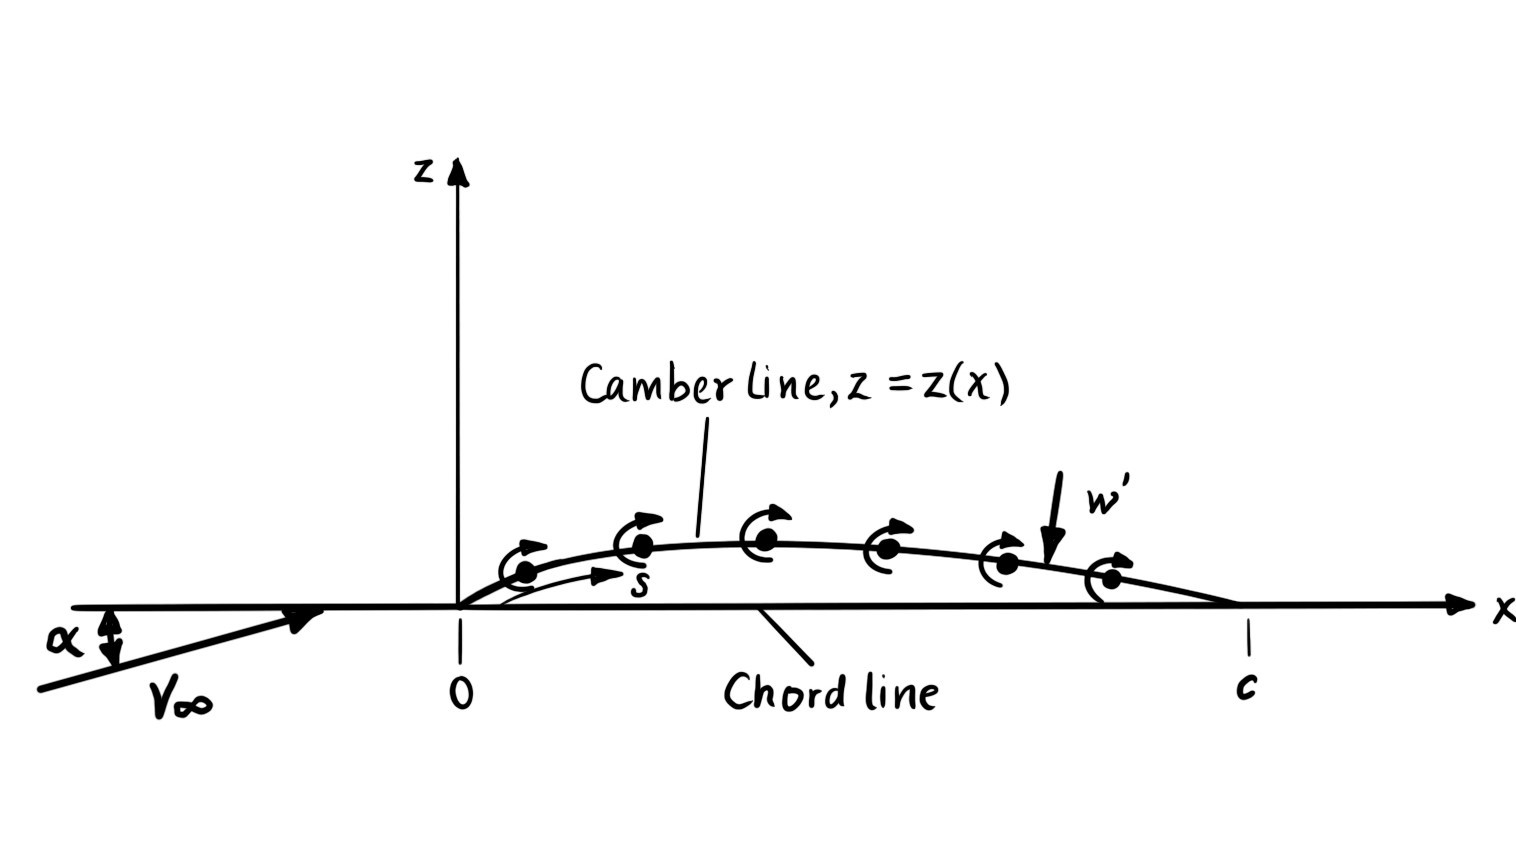
\includegraphics[scale=0.4]{1.1_vortexsheet_on_camber}
\centering
\caption{Vortex sheet placed on the camber line}
\label{v-camber}
\end{figure}

Consider a \textit{thin} airfoil in incompressible fluid flow with a freestream velocity $V_\infty$ and angle of attack $\alpha$. For \textit{thin} airfoils, a reasonable assumption we can make is that a vortex sheet placed on the surface of the airfoil can be approximated by a vortex sheet placed on the camberline, which in turn is the same as a vortex sheet placed on the chord line for moderate camber.

\begin{figure}[H]
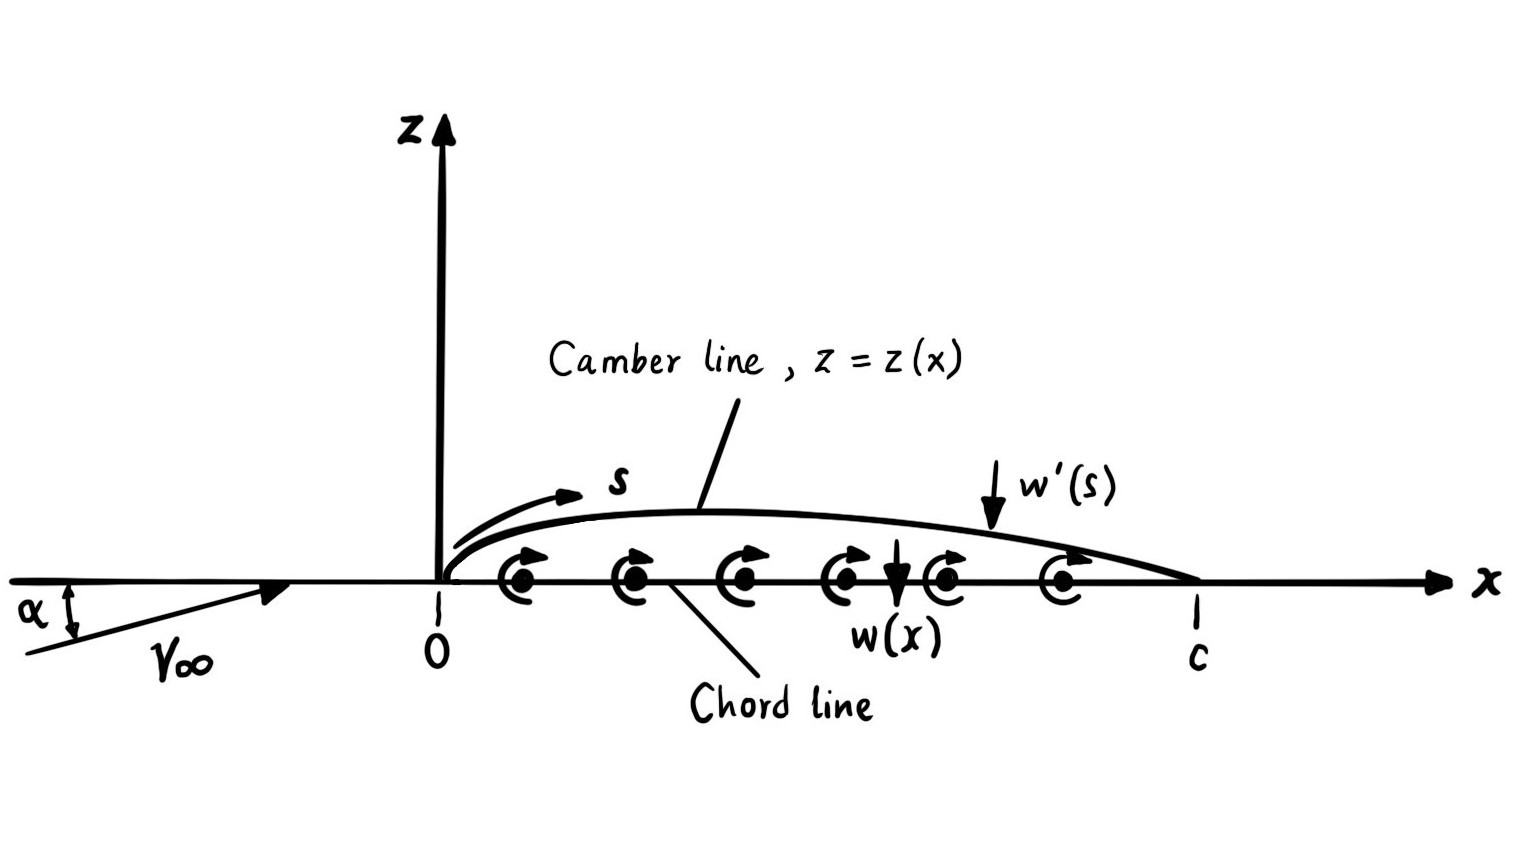
\includegraphics[scale=0.4]{1.2_vortexsheet_on_chord}
\centering
\caption{Vortex sheet placed on the chord line}
\label{v-chord}
\end{figure}

As shown in figures \ref{v-camber} and \ref{v-chord}, the \textit{x axis} falls on the chord line and \textit{z axis} is perpendicular to the chord. The chord length is \textit{c}. The camberline is defined by $z = z(x)$ and the distance measured along it is denoted by \textit{s}. When placed on the camberline, the vortex sheet induces velocity $\omega^{'}$ which is normal to the camber line; $\omega^{'} = \omega^{'}(s)$. Now, considering the vortex sheet is on the chord as shown in the figure \ref{v-chord}, here $\gamma = \gamma(x)$. The strength is calculated such that the camber line is a streamline of the flow and also $\gamma(c) = 0$ (satisfying Kutta condition).

If the camber line has to be a streamline of the flow, it means the component of velocity normal to the camber line must be zero at all points along the camber line. If the component of the freestream velocity normal to the camber line is denoted by $V_{\infty,n}$ then, at every point on the camber line 
\begin{equation}
V_{\infty,n} + \omega^{'}(s) = 0.
\label{v-norm}
\end{equation}

Now the normal component of freestream velocity can be determined simply by geometry. Refer figure \ref{norm-vel}. At any point where the slope is given by $dz/dx$, \[V_{\infty,n} = V_{\infty}  sin[ \alpha+tan^{-1}(-dz/dx) ]\]. Approximating $sin\theta \approx tan\theta \approx \theta$,
\begin{equation}
V_{\infty,n} = V_{\infty}\left(\alpha - \frac{dz}{dx}\right).
\label{v-inf-norm}
\end{equation}

\begin{figure}[H]
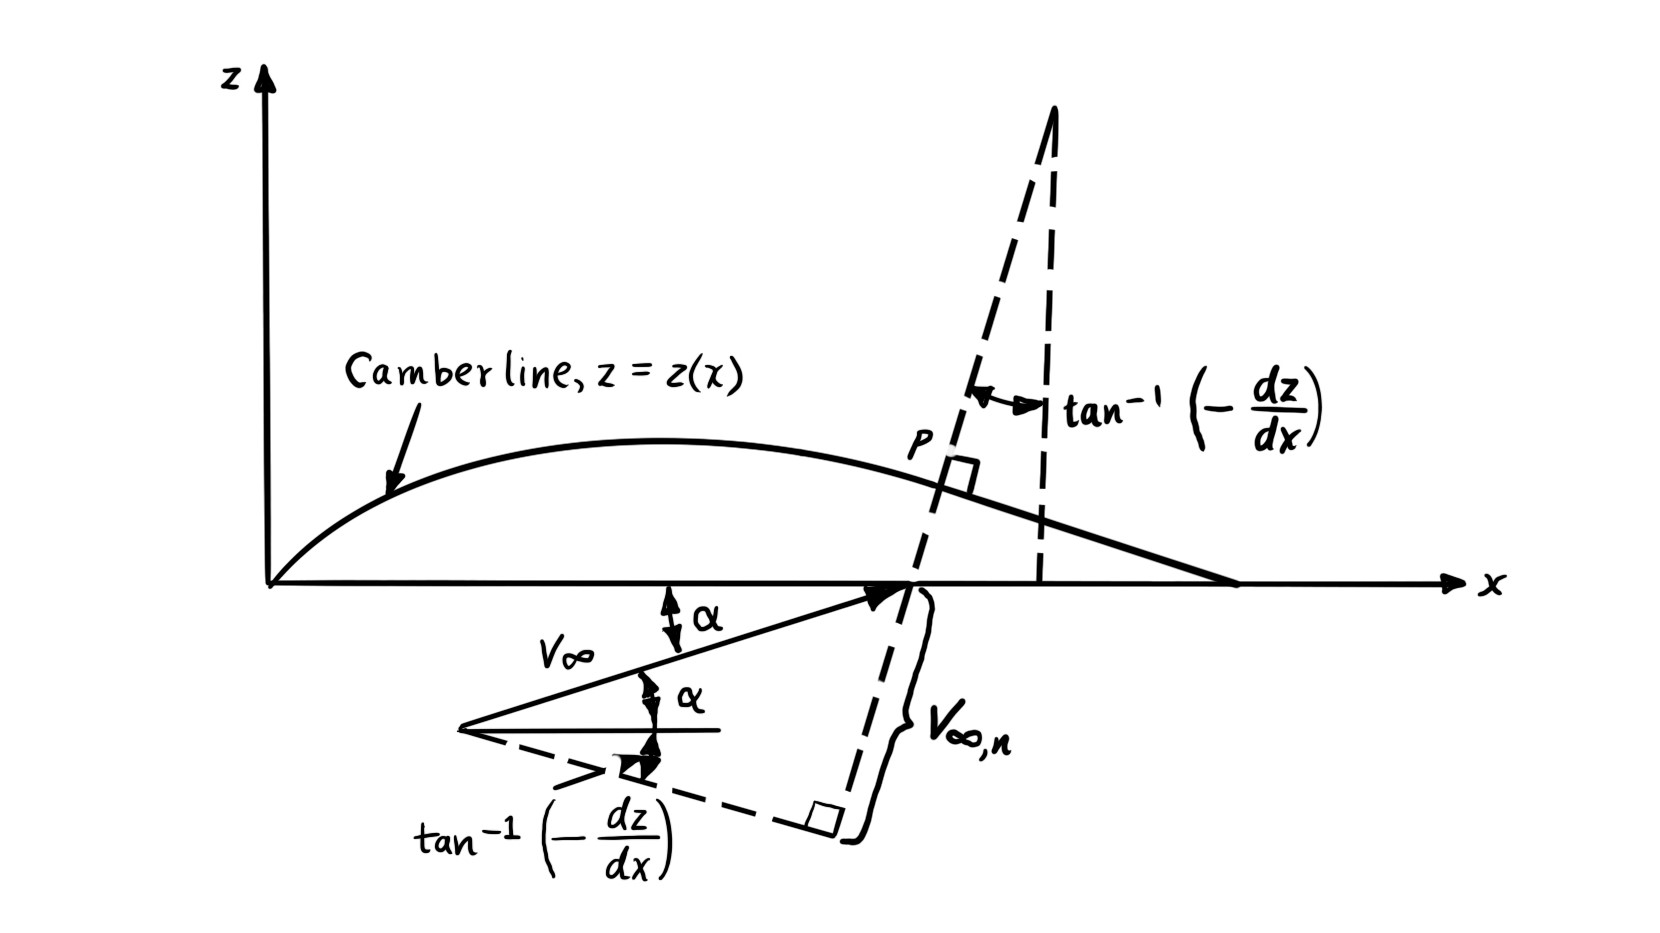
\includegraphics[scale=0.4]{1.3_v_infty}
\centering
\caption{Component of Freestream velocity normal to the camberline}
\label{norm-vel}
\end{figure}

Now we have to determine an expression for $\omega^{'}(s)$. Again, since we are dealing with \textit{thin} airfoils, the component of velocity (induced by the vortex sheet) normal to the camber line can be approximated to the component of the velocity normal to the chord line. \[\omega^{'}(s) \approx \omega(x)\].

\begin{figure}[H]
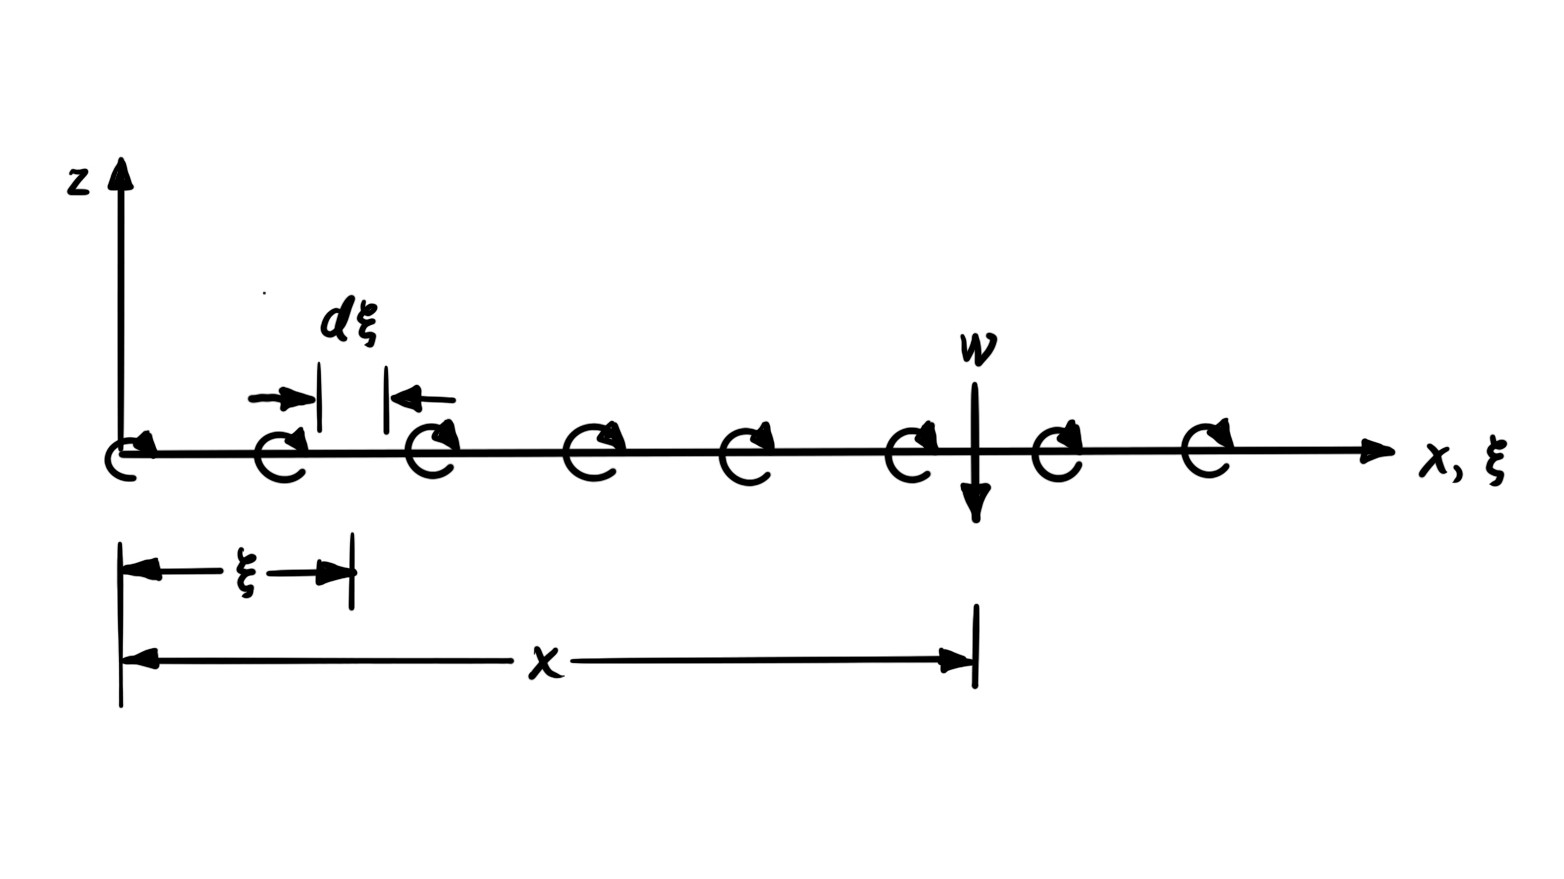
\includegraphics[scale=0.4]{1.4_vortexsheet_on_chord}
\centering
\caption{Induced velocity on the chord line}
\label{v-chord-2}
\end{figure}

To find an expression for $\omega(x)$, consider figure \ref{v-chord-2} which shows the vortex sheet along the chord. An elemental vortex of strength $\gamma d\xi$ is considered at an distance $\xi$ from the origin along the chord as shown. The strength of the vortex sheet is a function of the distance along the chord; i.e. $\gamma = \gamma(\xi)$.

The velocity $d\omega$ at point \textit{x} induced by this elemental vortex is given by
\begin{equation}
d\omega = -\frac{\gamma(\xi)d\xi}{2\pi(x-\xi)}.
\end{equation}
By integrating this expression from the leading edge ($\xi=0$) to the trailing edge ($\xi=c$), we can obtain $\omega(x)$ as
\begin{equation}
\omega(x)=- \int_{0}^{c} \frac{\gamma(\xi)d(\xi)}{2\pi(x-\xi)}
\label{omega-x}.
\end{equation}

Substituting equations \ref{v-inf-norm} and \ref{omega-x} in equation \ref{v-norm} we get
\begin{equation}
V_{\infty}\left(\alpha-\frac{dz}{dx}\right)-\int_{0}^{c} \frac{\gamma(\xi)d(\xi)}{2\pi(x-\xi)}=0,
\end{equation}
which is
\begin{equation}
\boxed{
\frac{1}{2\pi}\int_{0}^{c}\frac{\gamma(\xi)d(\xi)}{x-\xi}=V_{\infty}\left(\alpha-\frac{dz}{dx}\right).
}
\label{thin-airfoil}
\end{equation}
\textit{This is the fundamental equation of thin airfoil theory.}

It is imperative to note that for a given airfoil at a given angle of attack, both $\alpha$ and $dz/dx$ will be known. Hence, in equation \ref{thin-airfoil}, the vortex strength $\gamma(\xi)$ will be the only unknown. The critical step now is to solve this equation for $\gamma(\xi)$ such that it satisfies the Kutta condition, i.e. $\gamma(c)=0$.

Let\rq{}s take the case of a particular arbitrary airfoil. To deal with the integral in the fundamental equation, transform the variable $\xi$ to $\theta$ using the transformation
\[\xi=\frac{c}{2}(1-cos\theta)\].
Differentiating this, we get
\[d\xi=\frac{c}{2}sin\theta d\theta\].

The value of $x$ corresponds to a particular $\theta$, let it be $\theta_{0}$, such that 
\[x=\frac{c}{2}(1-cos\theta_{0})\].
The limits of the integration transform to $\theta=0$ when $\xi=0$ and $\theta=\pi$ when $\xi=c$.
Substituting all these in the equation, we get
\begin{equation}
\frac{1}{2\pi}\int_{0}^{\pi}\frac{\gamma(\theta)sin\theta d\theta}{cos\theta-cos\theta_{0}} = V_\infty\left(\alpha-\frac{dz}{dx}\right).
\label{eqncam}
\end{equation}
Equation \ref{eqncam} has to be solved for $\gamma(\theta)$, such that it satisfies the Kutta condition i.e. $\gamma(\pi)=0$. Such a solution will make the camber line a streamline of the flow. This solution is directly stated below
\begin{equation}\boxed{
\gamma(\theta)=2 V_\infty \left(A_{0}\frac{1+cos\theta}{sin\theta}+\sum_{n=1}^{\infty} A_{n}sinn\theta\right).
}
\label{eqngamma}
\end{equation}

The values of the coefficients, $A_{n}$ depends on the slope of the camber line $dz/dx$ and $A_{0}$ depends on both $dz/dx$ and $\alpha$.
Substituting equation $\ref{eqngamma}$ in equation $\ref{eqncam}$
\begin{equation}
\frac{1}{\pi}\int_0^\pi\frac{A_0(1+cos\theta) d\theta}{cos\theta-cos\theta_0}+\frac{1}{\pi}\sum_{n=1}^{\infty}\int_0^\pi\frac{A_n sinn\theta sin\theta d\theta}{cos\theta-cos\theta_0} = \alpha - \frac{dz}{dx}.
\label{eqncam2}
\end{equation}

Both the integral terms appearing above are forms of standard integrals which can be reduced as follows
\begin{equation}
\int_0^\pi\frac{cosn\theta d\theta}{cos\theta-cos\theta_0} = \frac{\pi sinn\theta_0}{sin\theta_0},
\end{equation}

\begin{equation}
\int_0^\pi\frac{sinn\theta sin\theta d\theta}{cos\theta-cos\theta_0} = -\pi cosn\theta_0.
\end{equation}

Hence equation $\ref{eqncam2}$ can be simplified to
\[
A_0 - \sum_{n=1}^{\infty}A_n cosn\theta_0 = \alpha - \frac{dz}{dx}
\]
or
\begin{equation}
\frac{dz}{dx} = (\alpha-A_0) + \sum_{n=1}^{\infty}A_n cosn\theta_0.
\label{dz}
\end{equation}

This equation is in the form of a Fourier cosine series. In general, Fourier cosine series of a function $f(\theta)$ over an interval $0\leq\theta\leq\pi$ is represented as
\begin{equation}
f(\theta) = B_0 + \sum_{n=1}^\infty B_n cosn\theta,
\end{equation}
where the coefficients are given by
\begin{align*}
B_0 &= \frac{1}{\pi}\int_0^\pi f(\theta) d\theta,\\
B_n &= \frac{2}{\pi}\int_0^\pi f(\theta) cosn\theta d\theta.
\end{align*}

Thus, the coefficients in equation \ref{dz} can be represented as
\[
(\alpha - A_0) = \frac{1}{\pi}\int\frac{dz}{dx}d\theta_0
\]
or
\begin{equation}
A_0 = \alpha - \frac{1}{\pi}\int_0^\pi\frac{dz}{dx}d\theta_0,
\label{A0}
\end{equation}

\begin{equation}
A_n = \frac{2}{\pi}\int_0^\pi\frac{dz}{dx}cosn\theta_0d\theta_0.
\label{AN}
\end{equation}

It can be seen from the expressions that $A_0$ depends on both $\alpha$ and the shape of the camberline($dz/dx$), and the values of $A_n$ depend only on the shape of the camberline. Hence, for a specific airfoil at a given angle of attack, the values of $A_0$ and $A_n$ can be calculated.

Next, we have to calculate the expressions for the aerodynamic coefficients. The total circulation due to the vortex sheet from the leading edge to the trailing edge is given by
\begin{equation}
\Gamma = \int_0^c\gamma(\xi)d\xi = \frac{c}{2}\int_0^\pi\gamma(\theta)sin\theta d\theta.
\label{circ}
\end{equation}

Substitute the expression of $\gamma(\theta)$ given by equation \ref{eqngamma} into equation \ref{circ}
\begin{equation}
\Gamma = cV_\infty \left(A_0\int_0^\pi(1+cos\theta)d\theta + \sum_{n=1}^\pi A_n\int_0^\pi sinn\theta sin\theta d\theta\right).
\label{circ2}
\end{equation}

From theory of integral calculus, we know
\[
\int_0^\pi (1+cos\theta)d\theta = \pi
\int_0^\pi sinn\theta sin\theta d\theta =
\begin{cases}
\pi/2 &for\ n=1\\
0 &for\ n\neq1
\end{cases}
\]
Hence equation \ref{circ2} becomes
\begin{equation}
\Gamma = cV_\infty \left(\pi A_0 + \frac{\pi}{2} A_1\right).
\end{equation}
Therefore, lift per unit span can be expressed as
\begin{equation}
L^{'} = \rho_\infty V_\infty \Gamma = \rho_\infty V_\infty^2 c \left(\pi A_0 + \frac{\pi}{2}A_1\right).
\end{equation}
Thus coefficient of lift can be expressed as
\begin{equation}
c_l = \frac{L^{'}}{\frac{1}{2}\rho_\infty V_\infty^2c(1)} = \pi(2A_0 + A_1).
\label{CL}
\end{equation}

which can be written as
\begin{equation}
\boxed{
c_l = 2\pi \left[\alpha + \frac{1}{\pi}\int_0^\pi \frac{dz}{dx}(cos\theta_0 - 1) d\theta_0\right],
}
\end{equation}
and
\begin{equation}
\boxed{
\text{Lift slope} \equiv \frac{dc_l}{d\alpha} = 2\pi.
}
\end{equation}
It is important to note that, irrespective of the airfoil characteristics, thin airfoil theory predicts that the value of the lift slope will always be $2\pi$.

Next, the moment about leading edge has to be calculated. As shown in figure \ref{LE-moment}, a elemental vortex of strength $\gamma(\xi)d\xi$ located at a distance of $\xi$ from the leading edge creates a circulation whose value is given by $d\Gamma = \gamma(\xi)d\xi$. So, the incremental lift created by this elemental vortex is $dL = \rho_\infty V_\infty d\Gamma$. This creates a moment about the leading edge $dM = -\xi(dL)$. 

\begin{figure}[h]
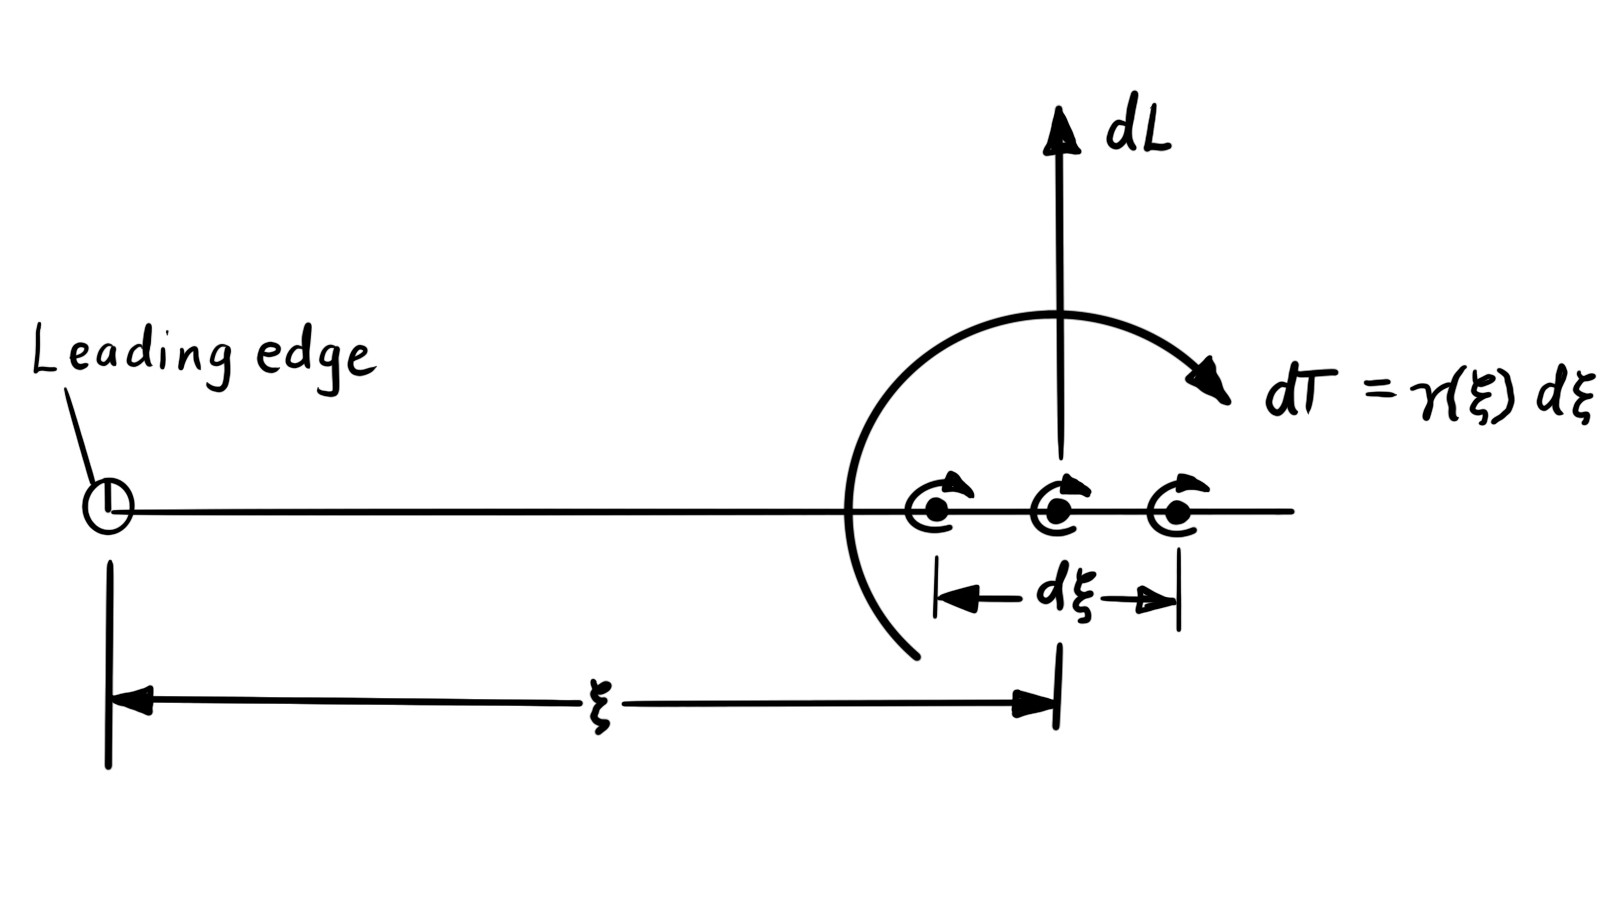
\includegraphics[scale=0.4]{1.5_moment_LE}
\centering
\caption{Moments about the leading edge}
\label{LE-moment}
\end{figure}

The total moment per unit span about the LE, therefore, can be calculated as
\begin{equation}
M_{LE}^{'} = -\int_0^c\xi(dL) = -\rho_\infty V_\infty \int_0^c\xi\gamma(\xi)d\xi.
\end{equation}

We also know the expression for the moment coefficient
\begin{equation}
c_{m,le} = \frac{M_{LE}^{'}}{q_{\infty}Sc}.
\end{equation}

Using similar transformation as was done before in the derivation of $\gamma(\theta)$ (equation \ref{eqngamma}), and performing the integration, and substituting $S = c * (1)$(considering unit depth), we get
\begin{equation}
c_{m,le} = -\frac{\pi}{2}\left(A_0+A_1-\frac{A_2}{2}\right).
\label{cmLE1}
\end{equation}
Substituting equation \ref{CL} in \ref{cmLE1}, we obtain
\begin{equation}
c_{m,le} = -\left[\frac{c_l}{4}+\frac{\pi}{4}(A_1-A_2)\right].
\label{cmLE}
\end{equation}

The moment coefficient about the quarter-chord point is given by
\begin{equation}
c_{m,c/4} = c_{m,le}+\frac{c_l}{4}.
\label{cmc4}
\end{equation}
Substituting equation \ref{cmLE} in equation \ref{cmc4}, we obtain
\begin{equation}
\boxed{
c_{m,c/4} = \frac{\pi}{4}(A_2-A_1).
}
\end{equation}

The location of the centre of pressure is given by
\begin{equation}
x_{cp} = -\frac{M_{LE}^{'}}{L^{'}} = -\frac{c_{m,le}c}{c_l}.
\end{equation}
Substituting the expression for $c_{m,le}$ from equation \ref{cmLE}, we can obtain the expression
\begin{equation}
\boxed{
x_{cp} = \frac{c}{4}\left[1+\frac{\pi}{c_l}(A_1-A_2)\right].
}
\end{equation}

\subsection{The Python Code}

\lstset{inputpath=./thin_airfoil/}
This section explains the crucial elements of the python code dealing with Thin Airfoi theory. The inputs given are geometry of the airfoil, specifically the coordinates of the camberline (`camberline.txt'), and the range of values of the angle of attack. The outputs are aerodynamic characteristics and several plots. Some snippets of the code are attached here with a brief contextual explanation. 

\lstinputlisting[firstline=116,lastline=120, caption=Input values]{thin_airfoil.py}

Towards the end of the code, you can find the values input for angle of attack, and the function `sweep' is called. This function is defined mainly to calculate the aerodynamic characteristics at each value of angle of attack. The function is defined as follows.

\lstinputlisting[firstline=51,lastline=82, caption=Sweep function]{thin_airfoil.py}

It can be noted here that the file camberline.txt is used to input the points of the camberline of the airfoil used, hence specifying the geometry. The other crucial part is calling of the function `thin\_airfoil'. This function is at the heart of the code, mainly specifying all the calculations of the aerodynamic coefficients. Some sections are discussed below.

\lstinputlisting[firstline=19,lastline=25, caption=$A_0$ and $A_n$ Coefficients]{thin_airfoil.py}

This section inside the function defined `thin\_airfoil' shows the calculation of each A[ ] coefficient clearly using the expressions obtained in equations \ref{A0} and \ref{AN}.

\lstinputlisting[firstline=27,lastline=33, caption=Circulation]{thin_airfoil.py}

This section calculates the values of $\gamma(\theta)$ by applying equation \ref{eqngamma}. The term is split into two loops with the nested loop taking care of the Sum($\Sigma$) expression.

\lstinputlisting[firstline=35,lastline=37, caption=Formulae]{thin_airfoil.py}
These lines are simply application of the various expressions obtained for $c_l$, $c_{m,c/4}$, $x_{cp}$ from the Thin airfoil theory.

\subsection{Test case}
The efficacy of any code can be judged by the comparison of the results from the code with experimental data. NACA 2412 airfoil has been taken as a test case, and the experimental data (obtained from reference \cite{naca}) has been compared and plotted as below. It can be observed that the results are fairly close.
\begin{figure}[H]
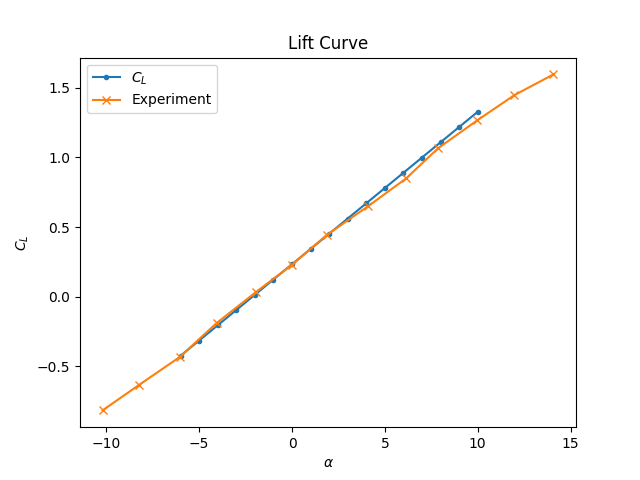
\includegraphics[scale=0.8]{1.6_cl_2412}
\centering
\caption{NACA2412 - $C_L$ vs $\alpha$}
\centering
\end{figure}

\begin{comment}   
\begin{minipage}{0.45\textwidth}
        \centering
        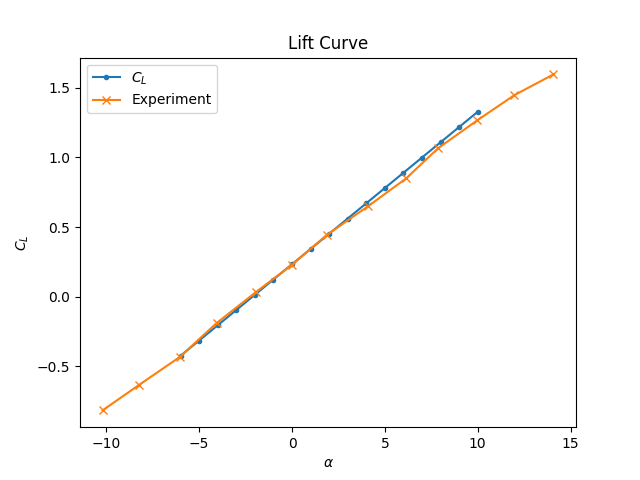
\includegraphics[scale=0.5]{1.6_cl_2412} % first figure itself
        \caption{Lift curve}
    \end{minipage}
    \begin{minipage}{0.45\textwidth}
        \centering
        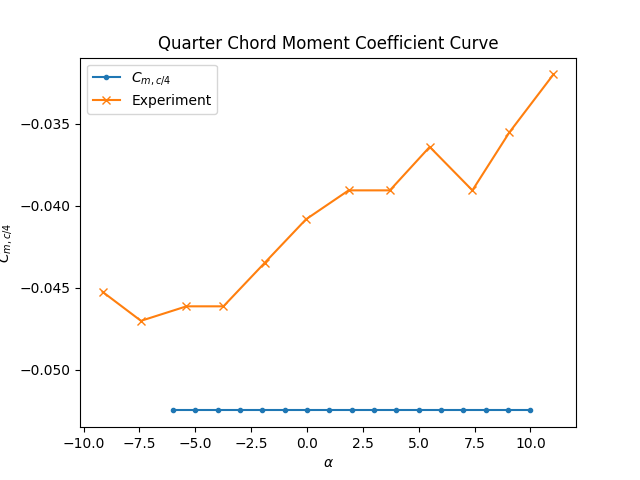
\includegraphics[scale=0.5]{1.7_cm_2412} % second figure itself
        \caption{Moment coefficient}
    \end{minipage}
\end{comment}

\begin{figure}[H]
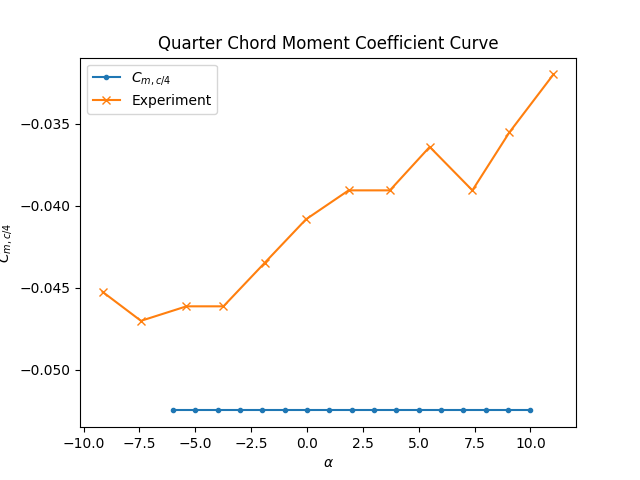
\includegraphics[scale=0.8]{1.7_cm_2412}
\centering
\caption{NACA2412 - Moment coefficient}
\end{figure}

\pagebreak%%%%%%%%

\section{Vortex Panel Method}
\subsection{Summary and Derivation \cite{chow}}

In this method, the airfoil considered is represented by a closed polygon comprised of vortex panels as shown in figure \ref{vortex-panel}. The number of panels is denoted by \textit{m}, they\rq{}re assumed to be planar and are named in clockwise direction starting from the trailing edge as shown in the figure. On each panel, the circulation density varies from one corner to the other in a linear fashion and is continuous across the corner.

\begin{figure}[H]
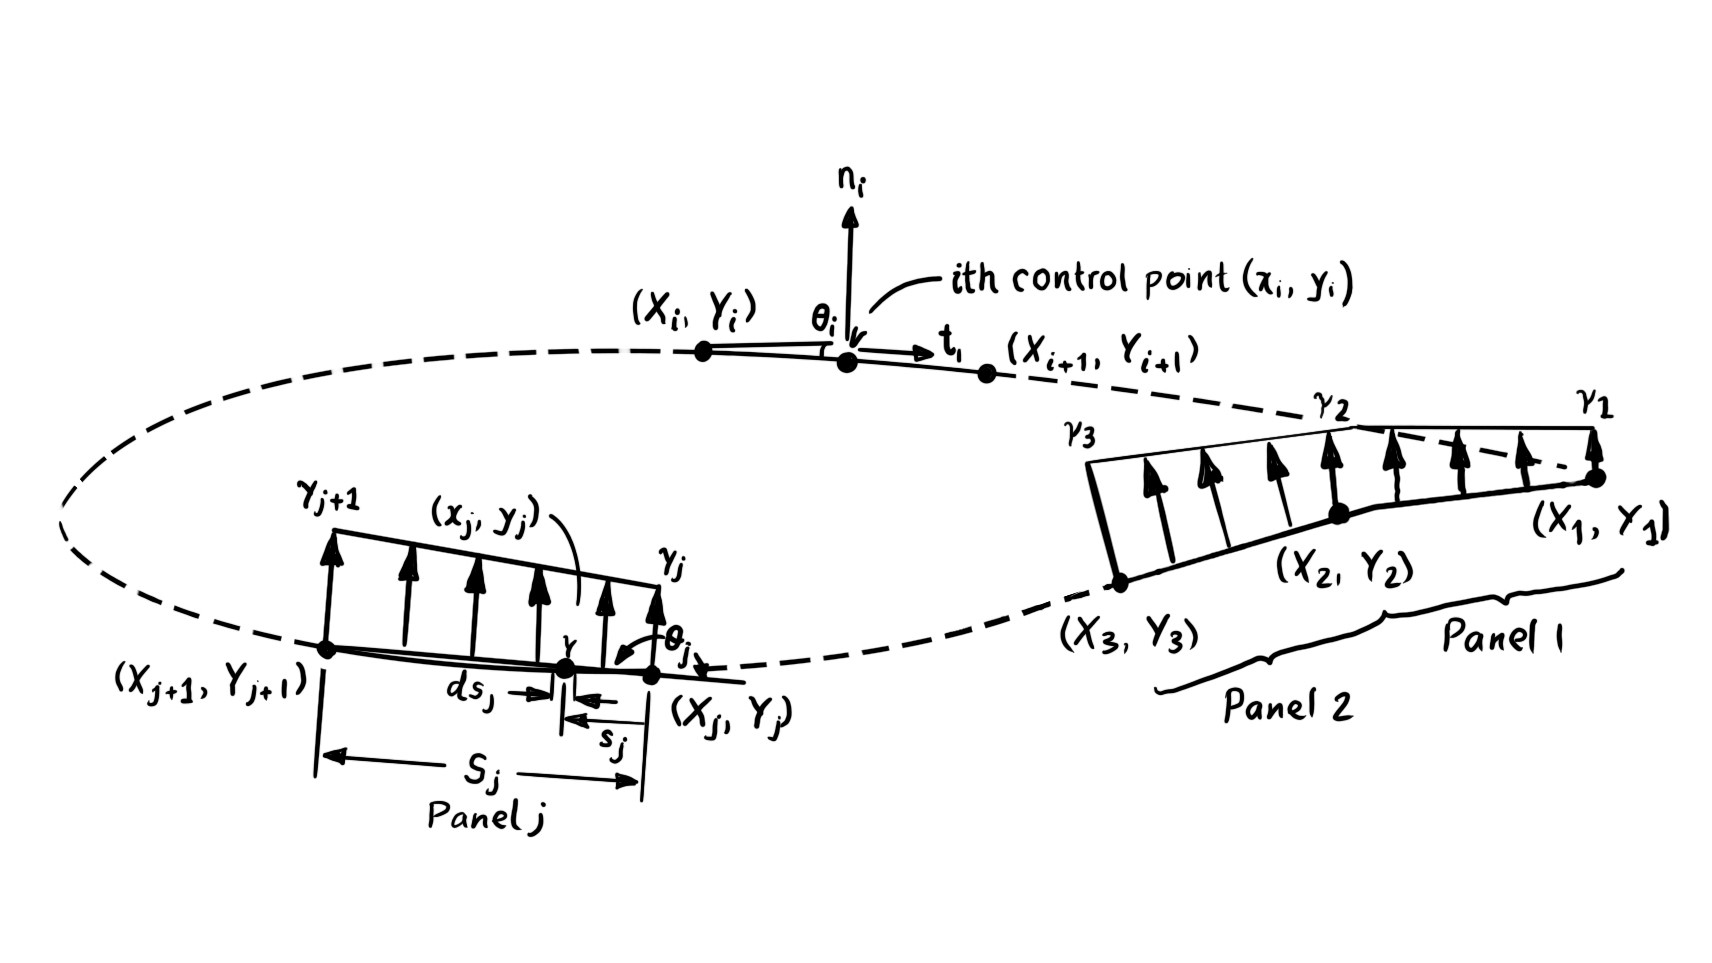
\includegraphics[scale=0.4]{2.1_panels}
\centering
\caption{Airfoil represented by Vortex panels}
\label{vortex-panel}
\end{figure}

The condition that the surface of the airfoil should be a streamline of the flow is satisfied by equating the normal component of velocity to zero at \textit{control points}, which are specified as the mid points of the panels. The end points of each panel are termed as the \textit{boundary points}.

The velocity potential $\phi$ at the \textit{i}th control point $(x_{i}, y_{i})$ is given by equation \ref{phi-xy}, where $V_{\infty}$ is the velocity of the uniform flow, $\alpha$ is the angle of attack, $m$ is the number of panels
\begin{equation}
\phi(x_{i}, y_{i}) = V_{\infty}(x_{i}cos\alpha+y_{i}sin\alpha) - \sum_{j=1}^{m}\int_{j}\frac{\gamma(s_{j})}{2\pi}tan^{-1}\left(\frac{y_{i}-y_{j}}{x_{i}-x_{j}}\right)ds_{j},
\label{phi-xy}
\end{equation}
where
\begin{equation}
\gamma(s_j) = \gamma_j+(\gamma_{j+1}-\gamma_j)\frac{s_j}{S_j}.
\end{equation}

Now, consider the boundary condition represented in figure \ref{vortex-panel}. It requires that the velocity in the direction of $n_i$, which is the unit vector directed outwards normal to the $i$th control panel, be equal to zero. So
\[
\frac{\partial}{\partial n_i}\phi(x_i, y_i)=0;\qquad i = 1,2,...,m
\].

Carrying out the differentiation steps, we finally obtain
\begin{equation}
\sum_{j=1}^m(C_{n1_{ij}}\gamma_j^{'}+C_{n2_{ij}}\gamma_{j+1}^{'}) = sin(\theta_i-\alpha);\qquad i = 1,2,...,m,
\label{norm}
\end{equation}
where $\gamma^{'} = \gamma/2\pi V_\infty$ is a dimensionless quantity representing circulation density, $\theta_i$ is the orientation angle of the $i$th panel which is the angle between the panel surface and $x$ axis and the coefficients are expressed as
\begin{align*}
&C_{n1_{ij}} = 0.5DF + CG - C_{n2_{ij}}\\
&C_{n2_{ij}} = D + 0.5QF/S_j - (AC + DE) G/S_j
\end{align*}.

These new constants in the above expressions are defined as
\begin{align*}
&A = -(x_i-X_j)cos\theta_j - (y_j-Y_j)sin\theta_j\\
&B = (x_i-X_j)^2 + (y_i-Y_j)^2\\
&C = sin(\theta_i-\theta_j)\\
&D = cos(\theta_i-\theta_j)\\
&E = (x_i-X_j)sin\theta_j - (y_i-Y_j)cos\theta_j\\
&F = ln\left(1+\frac{S_j^2+2AS_j}{B}\right)\\
&G = tan^{-1}\left(\frac{ES_j}{B+AS_j}\right)\\
&P = (x_i-X_j)sin(\theta_i-2\theta_j)+(y_i-Y_j)cos(\theta_i-2\theta_j)\\
&Q = (x_i-X_j)cos(\theta_i-2\theta_j)-(y_i-Y_j)sin(\theta_i-2\theta_j)
\end{align*}.

These constants can be calculated for all possible values of $i$ and $j$ once the panel geometry is specified.

The expression on the left hand side of equation $\ref{norm}$ enclosed in the parantheses denotes the normal velocity at the $i$th control point induced by the vortices on the $j$th panel. If we equate $i=j$, we get the self-induced normal velocity at the $i$th control point, the coefficients are simplied
\[
C_{n1_{ij}} = -1\qquad and\qquad C_{n2_{ij}} = 1.
\]

Now, the Kutta condition has to be applied to ensure a smooth flow at the trailing edge. In the present context, this condition (strength of the vorticity at the trailing edge equals zero) can be represented as
\begin{equation}
\gamma_1^{'} + \gamma_{m+1}^{'} = 0.
\label{kutta}
\end{equation}
Combining the equations $\ref{norm}$ and $\ref{kutta}$, we have $(m+1)$ number of equations which are sufficient to calculate $(m+1)$ number of unknown values of $\gamma_j^{'}$.

To facilitate in writing the code to implement this method, this system of simultaneous equations can be written in a more convenient form as
\begin{equation}
\sum_{j=1}^{m+1}A_{n_{ij}}\gamma_j^{'} = RHS_i;\qquad i = 1,2,..., m+1.
\end{equation}
Here, for $i\leq m+1$
\begin{align*}
A_{n_{i1}} &= C_{{n1}_{i1}}\\
A_{n_{ij}} &= C_{{n1}_{ij}} + C_{{n2}_{ij-1}};\qquad j = 2,3,...,m\\
A_{n_{im+1}} &= C_{{n2}_{im+1}}\\
RHS_i &= sin(\theta_i - \alpha)\\
\end{align*},
and, for $i=m+1$
\begin{align*}
A_{n_{i1}} &= A_{n_{im+1}} = 1\\
A_{n_{ij}} &= 0;\qquad j = 2,3,...,m\\
RHS_i &= 0\\
\end{align*}.



\subsection{Explanation of the code}
\lstset{inputpath=./vortex_panel/}
This section deals with a brief explanation of the code associated with the Vortex panel method. The input parameters are the geometry of the airfoil (via a .txt file containing the coordinates) and the range of values of angle of attack.

\lstinputlisting[firstline=148,lastline=155,caption=Input values]{vortex_panel.py}

Towards the end of the code, this section specifying the input parameters cna be found. It can be observed that loading the geometry here is performed by a function `load\_points'. The function can be found at the start of the code.
\lstinputlisting[firstline=6,lastline=30,caption=Specifying the geometry]{vortex_panel.py}
As shown, this function is defined to basically take the input text file and calculate the number of panels, centroids (mid points of the panels).

The function `sweep' which can be seen in the section dealing with input parameters is defined basically to calculate the values of $C_l$ for the different values of $\alpha$ .
\lstinputlisting[firstline=109,lastline=140,caption=Calculating $C_l$ for the range of angle of attack values]{vortex_panel.py}
It can be observed that the primary calculation of $C_l$ is carried out by calling the function `solve\_panel'. This function is crucial and at the heart of this code, and has all the calculations discussed in the theory.
\lstinputlisting[firstline=52,lastline=106,caption=Calculation of $C_l$]{vortex_panel.py}

The various coefficients are calculated here calling yet another function `coefficients'. This is defined before the `solve\_panel' function, and is basically the application of various expressions described after equation \ref{norm}.
\lstinputlisting[firstline=33,lastline=49,basicstyle=\small,columns=fullflexible,caption=Coefficients]{vortex_panel.py}

\subsection{Test case}
The results from the code agree well with the experimental data of NACA 2412 as shown in the plots below.
\begin{figure}[H]
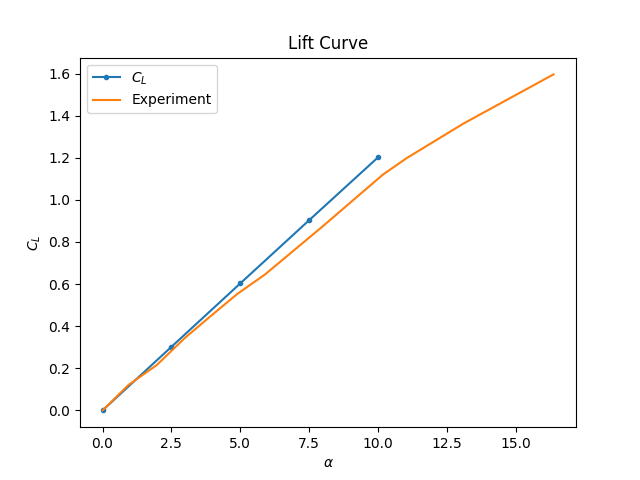
\includegraphics[scale=0.75]{2_cl}
\centering
\caption{NACA2412 - Lift curve}
\end{figure}
\begin{figure}[H]
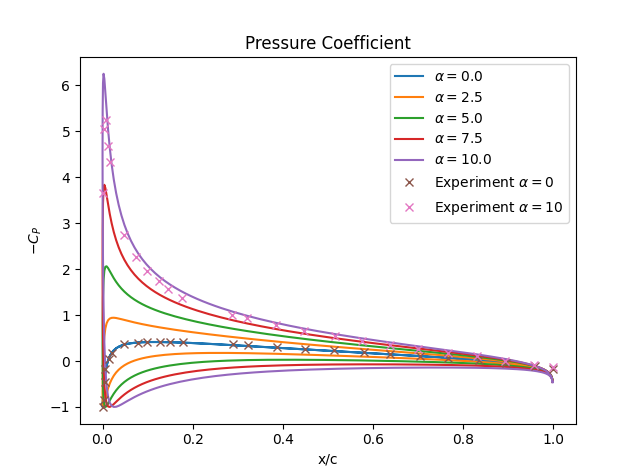
\includegraphics[scale=0.75]{2_cp}
\centering
\caption{NACA2412 - Pressure coefficient}
\end{figure}

\pagebreak%%%%%%%%%%

\section{Finite Wing - Prandtl's Classical Lifting-line Theory}
\subsection{Summary of the theory \cite{anderson}}
The previous theories dealt with airfoils, generally considered to have an `infinite' span. In practical applications however, all wings have a finite span. The finite wing theory analyses the characteristics differing from airfoil characteristics, like downwash, effective angle of attack, and induced drag.
The first successful theory to predict the aerodynamic properties of a wing is Prandtl's Lifting-line theory. It is explained briefly in this section with emphasis on obtaining the final expressions of the coefficients.

\begin{figure}[h]
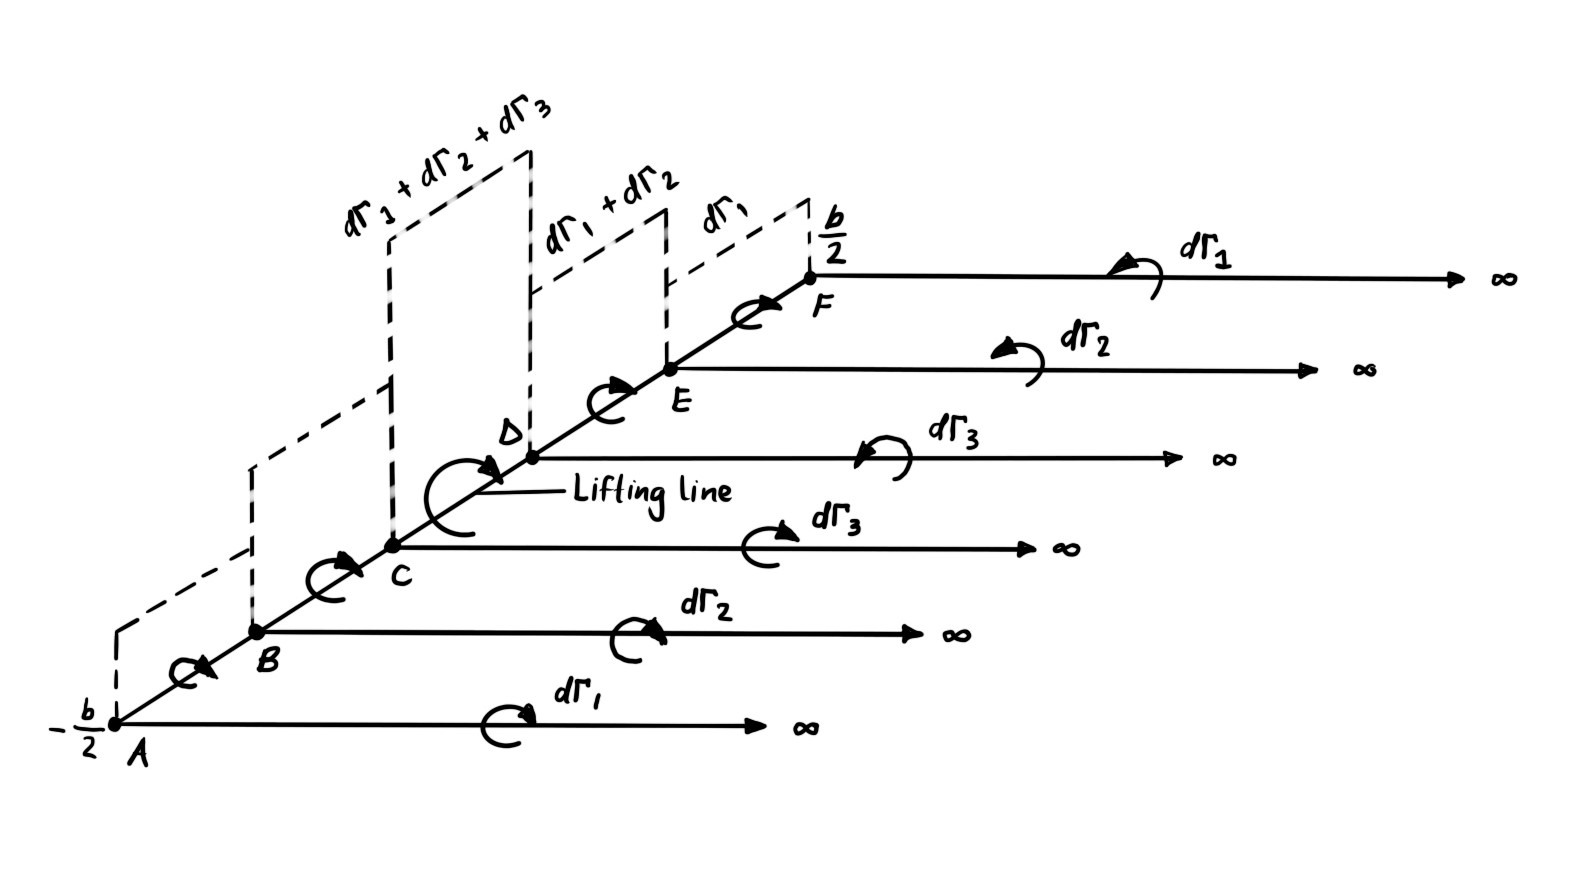
\includegraphics[scale=0.4]{3.1_finite_vortices}
\centering
\caption{Finite number of horseshoe vortices superimposed on lifting line}
\label{3.1}
\end{figure}

The wing is represented with a large number of horseshoe vortices, superimposed in such a way that all their bound vortices coincide along a single line, termed the \textit{lifting line}. The figure \ref{3.1} illustrates the concept showing just three vortices for clarity. It can be noted that there are trailing vortices distributed along the span and the strength of each trailing vortex is equal to the \textit{change in circulation} along the lifting line.

Now, assuming an infinite number of horseshoe vortices superimposed along the lifting line, each with infinitesimal strength $d\Gamma$. Here, the strength along the lifing line becomes a smooth distribution $\Gamma(y)$ with $\Gamma_0$ being the circulation at the origin. Also, trailing vortices here is a continuous vortex sheet trailing downstream. The total strength integrated across the span of the wing will be zero, because it consists of pairs of opposing vortices of equal strength.

\begin{figure}[h]
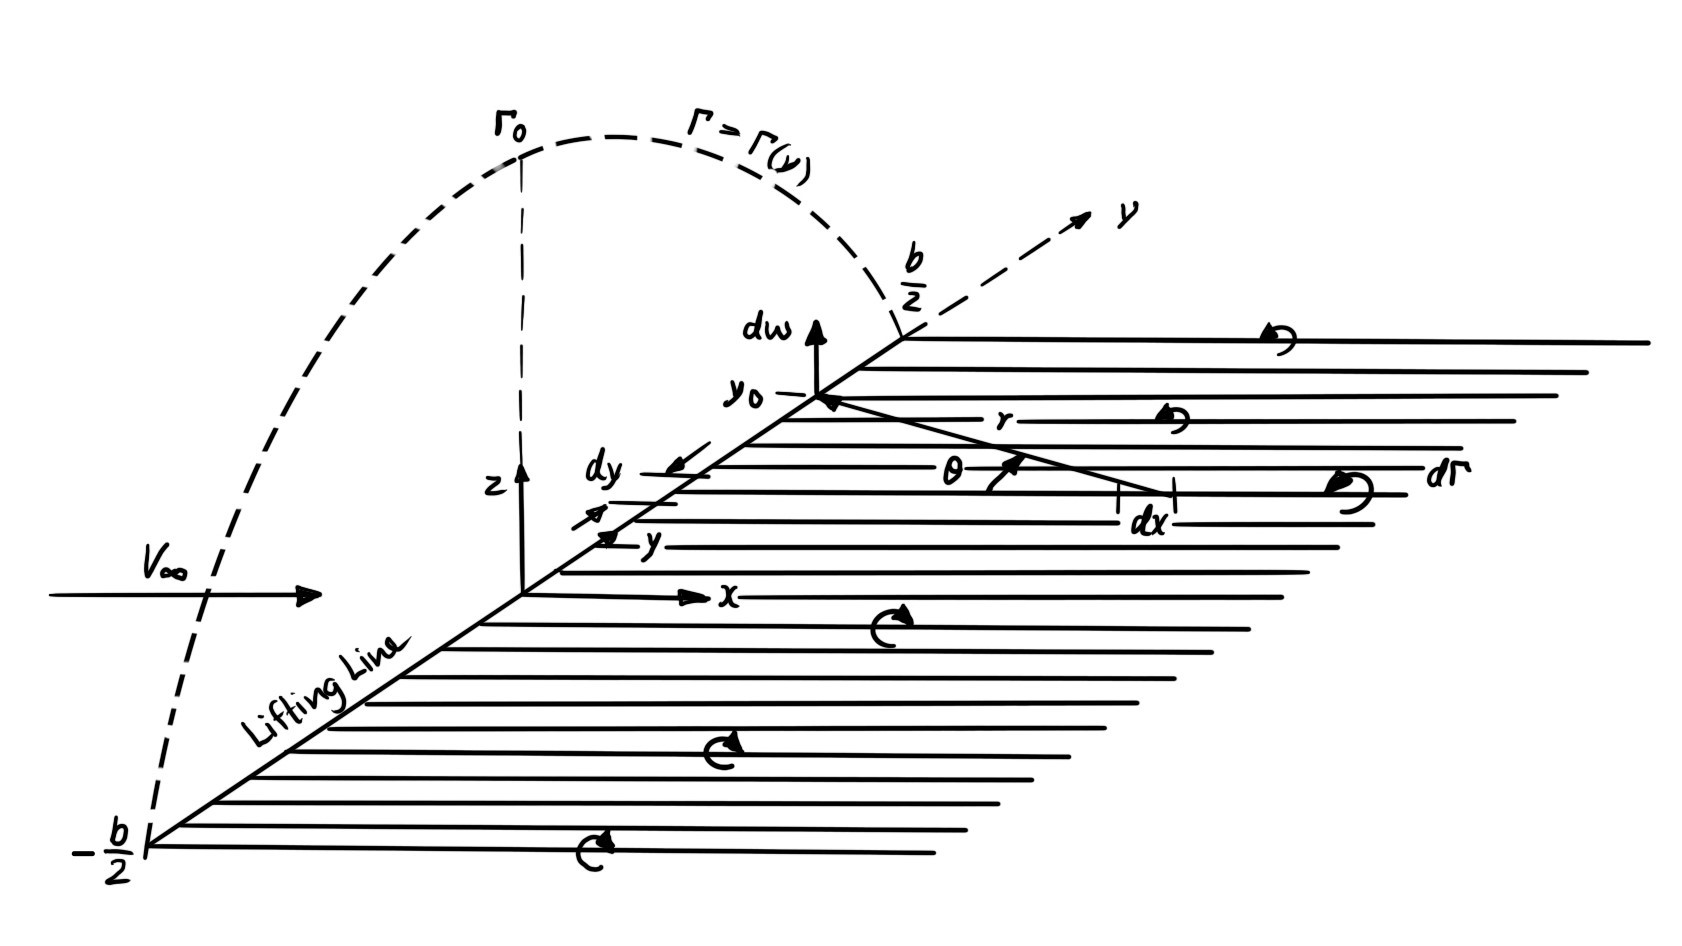
\includegraphics[scale=0.35]{3.2_infinite_vortices}
\centering
\caption{Infinite number of horseshoe vortices superimposed}
\label{3.2}
\end{figure}

Consider a small segment of the lifting line $dy$ located at a distance $y$ from the origin where the circulation is given by $\Gamma(y)$ and change in circulation over the segment is $d\Gamma = (d\Gamma/dy)dy$. Also, the strength of the trailing vortex must equal the change in the circulation $d\Gamma$ (as discussed in the case above). As shown in figure \ref{3.2}, consider a particular trailing vortex that intersects the lifting line at coordinate $y$, any segment $dx$ of this vortex will induce a velocity $d\omega$ at an arbitrary location on the lifting line $y_0$ such that
\begin{equation}
d\omega = -\frac{(d\Gamma/dy)dy}{4\pi(y_0-y)}.
\end{equation}

Integrating this equation from $-b/2$ to $b/2$, we can get the total velocity $\omega$ induced at $y_0$ by the entire traiing vortex sheet as
\begin{equation}
\omega(y_0) = -\frac{1}{4\pi}\int_{-b/2}^{b/2} \frac{(d\Gamma/dy)dy}{y_0-y}.
\end{equation}

The induced angle of attack (due to the downwash) at $y_0$ is given by
\begin{equation}
\alpha_i(y_0) = tan^{-1} \left(\frac{-\omega(y_0)}{V_\infty}\right).
\end{equation}
Usually, $\omega$ is much smaller than $V_\infty$ which means $\alpha_i$ is small enough to approximate
\begin{equation}
\alpha_i(y_0) = \frac{-\omega(y_0)}{V_\infty}.
\end{equation}
Substituting the value of $\omega(y_0)$, we get an expression for the induced angle of attack in terms of the circulation distribution along the wing as
\begin{equation}
\boxed{
\alpha_i(y_0) = \frac{1}{4\pi V_\infty}\int_{-b/2}^{b/2}\frac{(d\Gamma/dy)dy}{y_0-y}.
}
\label{indAOA}
\end{equation}

We know the relation between sectional coefficient of lift and effective angle of attack is given by
\begin{equation}
c_l = a_0[\alpha_{\text{eff}}(y_0)-\alpha_{L=0}] = 2\pi[\alpha_{\text{eff}}(y_0)-\alpha_{L=0}].
\end{equation}

Two different expressions for Lift (per unit span) are considered, one by definition of lift coefficient and second from Kutta-Joukowski theorem
\begin{equation}
L^{'} = 1/2\rho_\infty V_\infty^2c(y_0)c_l = \rho_\infty V_\infty\Gamma(y_0).
\end{equation}

This gives us an expression for $c_l$
\begin{equation}
c_l = \frac{2\Gamma(y_0)}{V_\infty c(y_0)}.
\end{equation}

Solving for $\alpha_{\text{eff}}$, we get
\begin{equation}
\alpha_{\text{eff}} = \frac{\Gamma(y_0)}{\pi V_\infty c(y_0)}+\alpha_{L=0}.
\end{equation}

We also know, from definition
\begin{equation}
\alpha_{\text{eff}} = \alpha-\alpha_i.
\end{equation}

Therefore, solving for geometric angle of attack at $y_0$, we obtain
\begin{equation}
\boxed{
\alpha(y_0) = \frac{\Gamma(y_0)}{\pi V_\infty c(y_0)}+\alpha_{L=0}(y_0)+\frac{1}{4\pi V_\infty}\int_{-b/2}^{b/2}\frac{(d\Gamma/dy)dy}{y_0-y}.
}
\label{prandtl}
\end{equation}
This is the \textit{fundamental equation of Prandtl's lifting-line theory}. It should be noted that the only unknown in this equation is $\Gamma$; all the other terms are known for a given wing design at a given geometric angle of attack in a flow with a given freestream velocity. Thus solution of Equation \ref{prandtl} gives us the circulation function $\Gamma = \Gamma(y_0)$, where $y_0$ ranges from $-b/2$ to $b/2$. This, in turn, gives us the Lift, Coefficient of lift and Induced drag.

We proceed by assuming a general circulation distribution in the form of a Fourier sine series considering the following transformation of coordinates
\begin{equation}
y = -\frac{b}{2}cos\theta.
\end{equation}

So, the coordinate along the wing span is now $\theta$, $0\leq\theta\leq\pi$; the circulation distribution is assumed as
\begin{equation}
\Gamma(\theta) = 2bV_\infty\sum_1^NA_nsinn\theta.
\label{general}
\end{equation}
where N is the number of terms in the Fourier series, higher number of terms gives higher accuracy. Differentiating this equation, we obtain
\begin{equation}
\frac{d\Gamma}{dy} = \frac{d\Gamma}{d\theta}\frac{d\theta}{dy} = 2bV_\infty\sum_1^NnA_ncosn\theta\frac{d\theta}{dy}.
\end{equation}

Substituting these expressions of $\Gamma$ and $d\Gamma/dy$ in the fundamental equation, we obtain
\begin{equation}
\boxed{
\alpha(\theta_0) = \frac{2b}{\pi c(\theta_0)}\sum_1^NA_nsinn\theta_0+\alpha_{L=0}(\theta_0)+\sum_1^NnA_n\frac{sinn\theta_0}{sin\theta_0}.
}
\label{GAOA}
\end{equation}

It can be observed that, for a given span location ($\theta_0$ is specified), the only unknowns in equation \ref{GAOA} are the N number of coefficients $A_n$s. So, if we take N different locations along the span and evaluate Equation \ref{GAOA} for each of these N locations, we end up with a system of N independent algebraic equations with N unknowns (the coefficients). Solving this system, we can obtain all the values for the $A_n$s. Hence, the general circulation distribution $\Gamma(\theta)$ can be obtained. The lift coefficient follows.

Lift per span distribution is given by Kutta-Joukowski theorem (in terms of span length coordinate $y$) as
\begin{equation}
L^{'}(y_0) = \rho_\infty V_\infty \Gamma(y).
\end{equation}

The total lift can be obtained by integrating this equation over the span, hence
\begin{equation}
L = \rho_\infty V_\infty\int_{-b/2}^{b/2}\Gamma(y)dy.
\end{equation}
Then the lift coefficient, by definition, will be given by
\begin{equation}
C_L = \frac{L}{q_\infty S} = \frac{2}{V_\infty}\int_{-b/2}^{b/2}\Gamma(y)dy.
\end{equation}

Substituting the expression we assumed for the general circulation distribution, equation \ref{general}, we get
\begin{equation}
C_L = \frac{2b^2}{S}\sum_1^NA_n\int_0^\pi sinn\theta sin\theta d\theta.
\end{equation}
Here, the integral can be evaluated as
\[
\int_0^\pi sinn\theta sin\theta d\theta =
\begin{cases}
\pi/2 &for\ n=1\\
0 &for\ n \neq 1
\end{cases}
\].

Hence, the lift coefficient simplifies to
\begin{equation}
C_L = A_1\pi\frac{b^2}{S} = A_1\pi AR.
\label{CoeffL}
\end{equation}

Next, moving on to induced drag coefficient. It follows from definition of Induced drag (assuming induced angle is small)
\begin{equation}
D_i^{'} = L^{'}\alpha_i.
\end{equation}
Total induced drag is obtained by integrating this expression over the span, hence
\begin{equation}
D_i = \int_{-b/2}^{b/2}L^{'}(y)\alpha_i(y)dy.
\end{equation}

The induced drag coefficient is given by
\begin{equation}
C_{D,i} = \frac{D_i}{q_\infty S} = \frac{2}{V_\infty S}\int_{-b/2}^{b/2}\Gamma(y)\alpha_i(y)dy.
\end{equation}

Now, substituting our assumed expression for the circulation, i.e. equation \ref{general}, we get
\begin{equation}
C_{D,i} = \frac{2b^2}{S}\int_0^\pi\left(\sum_1^NA_nsinn\theta\right)\alpha_i(\theta)sin\theta d\theta.
\label{cdi1}
\end{equation}

The expression for induced angle of attack can be obtained from equation \ref{indAOA}
\begin{equation}
\alpha_i(y_0) = \frac{1}{4\pi V_\infty}\int_{-b/2}^{b/2}\frac{(d\Gamma/dy)dy}{y_0-y} = \frac{1}{\pi}\sum_1^NnA_n\int_0^\pi\frac{cosn\theta}{cos\theta-cos\theta_0}d\theta.
\end{equation}

Solving the integral using its standard form, we get
\begin{equation}
\alpha_i(\theta_0) = \sum_1^NnA_n\frac{sinn\theta_0}{sinn\theta_0},
\end{equation}
which can also be written as
\begin{equation}
\alpha_i(\theta) = \sum_1^NnA_n\frac{sinn\theta}{sinn\theta}.
\end{equation}

Hence, equation \ref{cdi1} becomes
\begin{equation}
C_{D,i} = \frac{2b^2}{S}\int_0^\pi\left(\sum_1^NA_nsinn\theta\right)\left(\sum_1^NnA_nsinn\theta\right)d\theta.
\label{cdi2}
\end{equation}

This equation involves the \textit{product} of two summations. From the standard integral
\begin{equation}
\int_0^\pi sinm\theta sink\theta =
\begin{cases}
0 &for\ m\neq k\\
\pi/2 &for\ m=k
\end{cases}.
\end{equation}

This means all the mixed product terms having unequal subscripts (like $A_1A_2$,$A_2A_4$ etc) in equation \ref{cdi2} reduce to zero, simplifying it to
\begin{align*}
C_{D,i} &= \frac{2b^2}{S}\left(\sum_1^NnA_n^2\right)\frac{\pi}{2} = \pi AR\sum_1^NnA_n^2\\
&= \pi AR\left(A_!^2+\sum_2^NnA_n^2\right)
\end{align*},
\begin{equation}
= \pi AR A_1^2\left[1+\sum_2^Nn{\left(\frac{A_n}{A_1}\right)}^2\right].
\end{equation}

Substituting the value of $C_L$ obtained in equation \ref{CoeffL}, we get
\begin{equation}
\boxed{
C_{D,i} = \frac{C_L^2}{\pi AR}(1+\delta),
}
\label{cdi3}
\end{equation}
where $\delta = \sum_2^Nn(A_n/A_1)^2$. Now, defining a \textit{span efficiency factor} as $e = (1+\delta)^{-1}$, equation \ref{cdi3} becomes
\begin{equation}
\boxed{
C_{D,i} = \frac{C_L^2}{\pi eAR}.
}
\end{equation}


\subsection{Explanation of the code}
\lstset{inputpath=./finite_wing/}

The input parameters here are Wingspan, Chord length in terms of spanwise location, Geometric angle of attack, Zero-lift angle of attack, Number of terms in the expansion(affects accuracy of the results).

\lstinputlisting[firstline=182,lastline=193,caption=Input values]{finite_wing.py}

Towards the end of the code, you can find the input parameters defined. It can be seen that two functions have been called here. The `drag\_polar' function simply does the function of calculating $C_L$ and $C_{D_i}$ for the range of angle of attack values and plotting them. The crucial function which performs these calculations following the theory discussed above is the `finite\_wing' function. A few sections are discussed below. 

\lstinputlisting[firstline=47,lastline=62,caption=$A_n$ Coefficients]{finite_wing.py}

The equations written here to generate the coefficient matrix is obtained from Equation \ref{GAOA}, solving a system of $N$ number of independent algebraic equations to get the $N$ number of coefficients. These values are stored in the `An' array.

\lstinputlisting[firstline=64,lastline=76,caption=Calculating Lift and Drag Coefficients]{finite_wing.py}
The computation of lift and drag coefficients here are straighforward applications of the expressions obtained in the theory, equations \ref{CoeffL} and \ref{cdi3}.
\lstinputlisting[firstline=83,lastline=88,caption=Calculating Circulation]{finite_wing.py}
The computation of circulation is a direct application of the general expression we assumed, equation \ref{general}.

\subsection{Validation}
For validating the Finite wing code, two different plots were used from the relevant section of reference \cite{anderson}. First, circulation distribution generated using a \textit{Numerical Non-linear method} for rectangular wings of aspect ratios 4 and 8 (NACA 1412) are compared with the values obtained from the code. Excellent agreement can be observed, as shown in figures \ref{finite-ar4} and \ref{finite-ar8}. Further, figure \ref{finite-cl} shows comparison of values of $C_L$ for a rectangular wing of aspect ratio 5.536 (NACA 0015).

\begin{figure}[H]
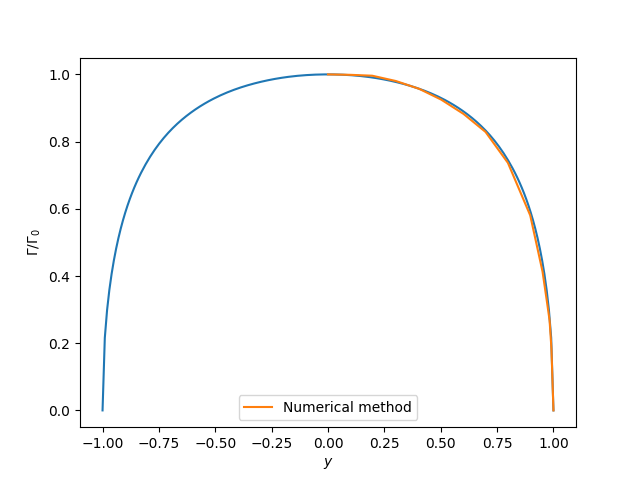
\includegraphics[scale=0.8]{finite_gamma_1412_ar4}
\centering
\caption{Comparison of $\Gamma/\Gamma_0$ for a rectangular wing of AR 4 (NACA1412)}
\label{finite-ar4}
\end{figure}

\begin{figure}[H]
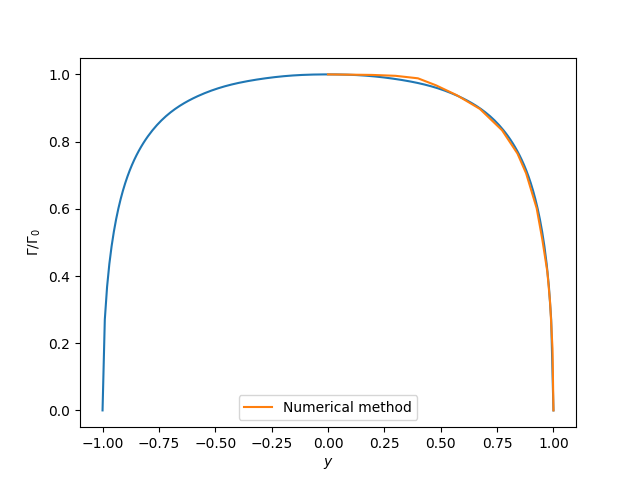
\includegraphics[scale=0.75]{finite_gamma_1412_ar8}
\centering
\caption{Comparison of $\Gamma/\Gamma_0$ for a rectangular wing of AR 8 (NACA1412)}
\label{finite-ar8}
\end{figure}

\begin{figure}[H]
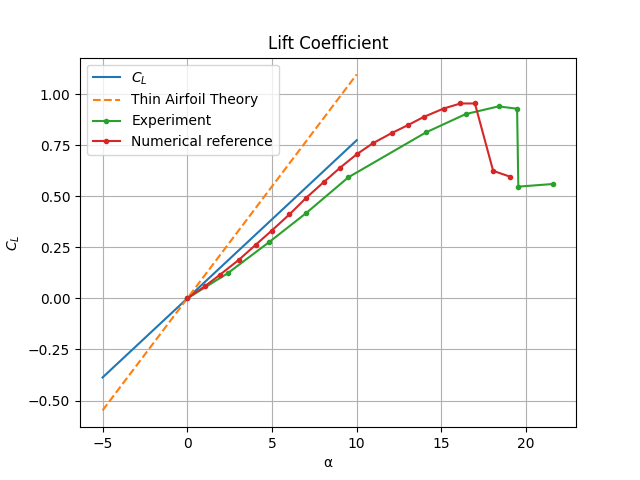
\includegraphics[scale=0.75]{finite_CL_0015}
\centering
\caption{Comparison of $C_L$ for a rectangular wing of AR 5.536 (NACA0015)}
\label{finite-cl}
\end{figure}

\pagebreak%%%%%%%%

\section{Performance}
\subsection{Summary of the theory involved \cite{phillips}}
\subsubsection{General performance parameters}
\paragraph{Thrust required}

First we are going to discuss the thrust required to maintain \textit{steady}, \textit{level} flight. \textit{Steady} flight means the aircraft is at a constant speed i.e. no acceleration and \textit{level} flight means both climb angle and bank angle are zero i.e. there is no change in altitude. The thrust required is a function of airspeed, altitude, size, shape, and weight of the aircraft. The forces acting on an aircraft in steady, level flight is shown in figure \ref{forces-level}.

\begin{figure}[h]
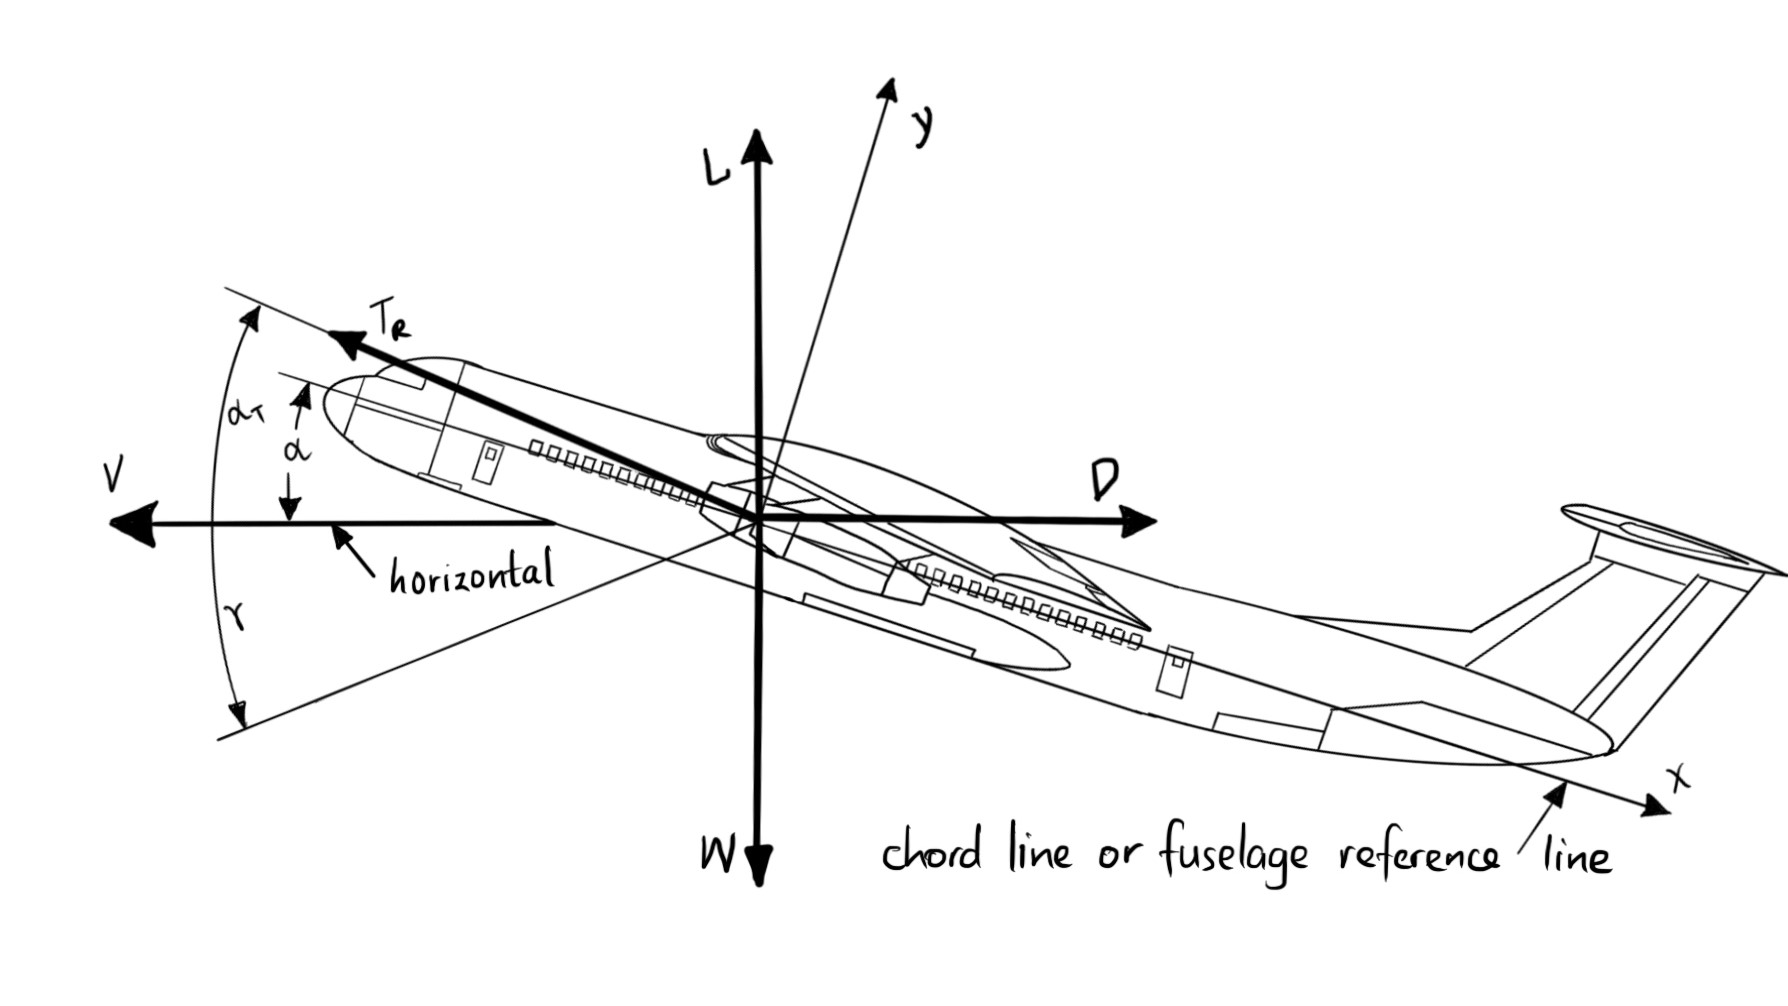
\includegraphics[scale=0.4]{forces_level}
\centering
\caption{Forces acting on an aircraft in level flight}
\label{forces-level}
\end{figure}

Since there is no acceleration, the drag force equals the thrust component in the direction of flight
\begin{equation}
D=T_Rcos\alpha_T.
\end{equation}

The lift must equal the weight minus the thrust component perpendicular to the direction of flight
\begin{equation}
L=W-T_Rsin\alpha_T.
\label{lift1}
\end{equation}

From these two equations, it is apparent that
\begin{equation}
\frac{L}{D}=\frac{W-T_Rsin\alpha_T}{T_Rcos\alpha_T}.
\end{equation}
or, solving for the expression for Thrust required
\begin{equation}
T_R=\frac{W}{(L/D)cos\alpha_T+sin\alpha_T}.
\label{thrust1}
\end{equation}

Now, the total drag force, which is the sum of parasitic drag and induced drag, can be written as
\begin{equation}
D=\frac{1}{2}\rho V^2S_wC_D = \frac{1}{2}\rho V^2 S_w\left(C_{D_p}+\frac{C_L^2}{\pi e_sR_A}\right),
\label{drag1}
\end{equation}
where $V$ is the airspeed, $S_w$ is the area of the main wing, $e_s$ is the span efficiency factor, $R_A$ is the aspect ratio, and $C_{D_p}$ represents the parasitic drag coefficient. $C_{D_p}$ can be written as a parabolic function of $C_L$
\begin{equation}
C_{D_p}=C_{D_0}+C_{{D_0},L}C_L+C_{{D_0},{L^2}}C_L^2.
\label{cdp}
\end{equation}

Substituting equation \ref{cdp} in equation \ref{drag1} and combining the quadratic term from the expression for the parasitic drag with the induced drag term, the total drag can be expressed as
\begin{equation}
D=\frac{1}{2}\rho V^2S_w\left(C_{D_0}+C_{{D_0},L}C_L+\frac{C_L^2}{\pi eR_A}\right).
\label{drag2}
\end{equation}
Here $e$ is the Oswald efficiency factor. Therefore
\begin{equation}
\boxed{
\frac{L}{D}=\frac{C_L}{C_D}=\frac{C_L}{C_{D_0}+C_{{D_0},L}C_L+\frac{C_L^2}{\pi eR_A}}.
}
\label{LDratio}
\end{equation}

Substituting equation \ref{lift1} in the definition of $C_L$, we have
\begin{equation}
C_L=\frac{L}{\frac{1}{2}\rho V^2S_w}=\frac{W-T_R sin\alpha_T}{\frac{1}{2}\rho V^2S_w}.
\end{equation}

Using the expression for Thrust required from \ref{thrust1}
\begin{equation}
\boxed{
C_L=\frac{W}{\frac{1}{2}\rho V^2S_w}\left[1-\frac{sin\alpha_T}{(L/D)cos\alpha_T+sin\alpha_T}\right]=\frac{W}{\frac{1}{2}\rho V^2S_w}\left[\frac{1}{1+(D/L)tan\alpha_T}\right].
}
\label{cl1}
\end{equation}

Using the equations \ref{LDratio} and \ref{cl1}, both $C_L$ and $L/D$ as a function of airspeed can be determined numerically. A typical example of a plot of lift-drag ratio versus airspeed is shown in figure \ref{LDRvsV}.
\begin{figure}[H]
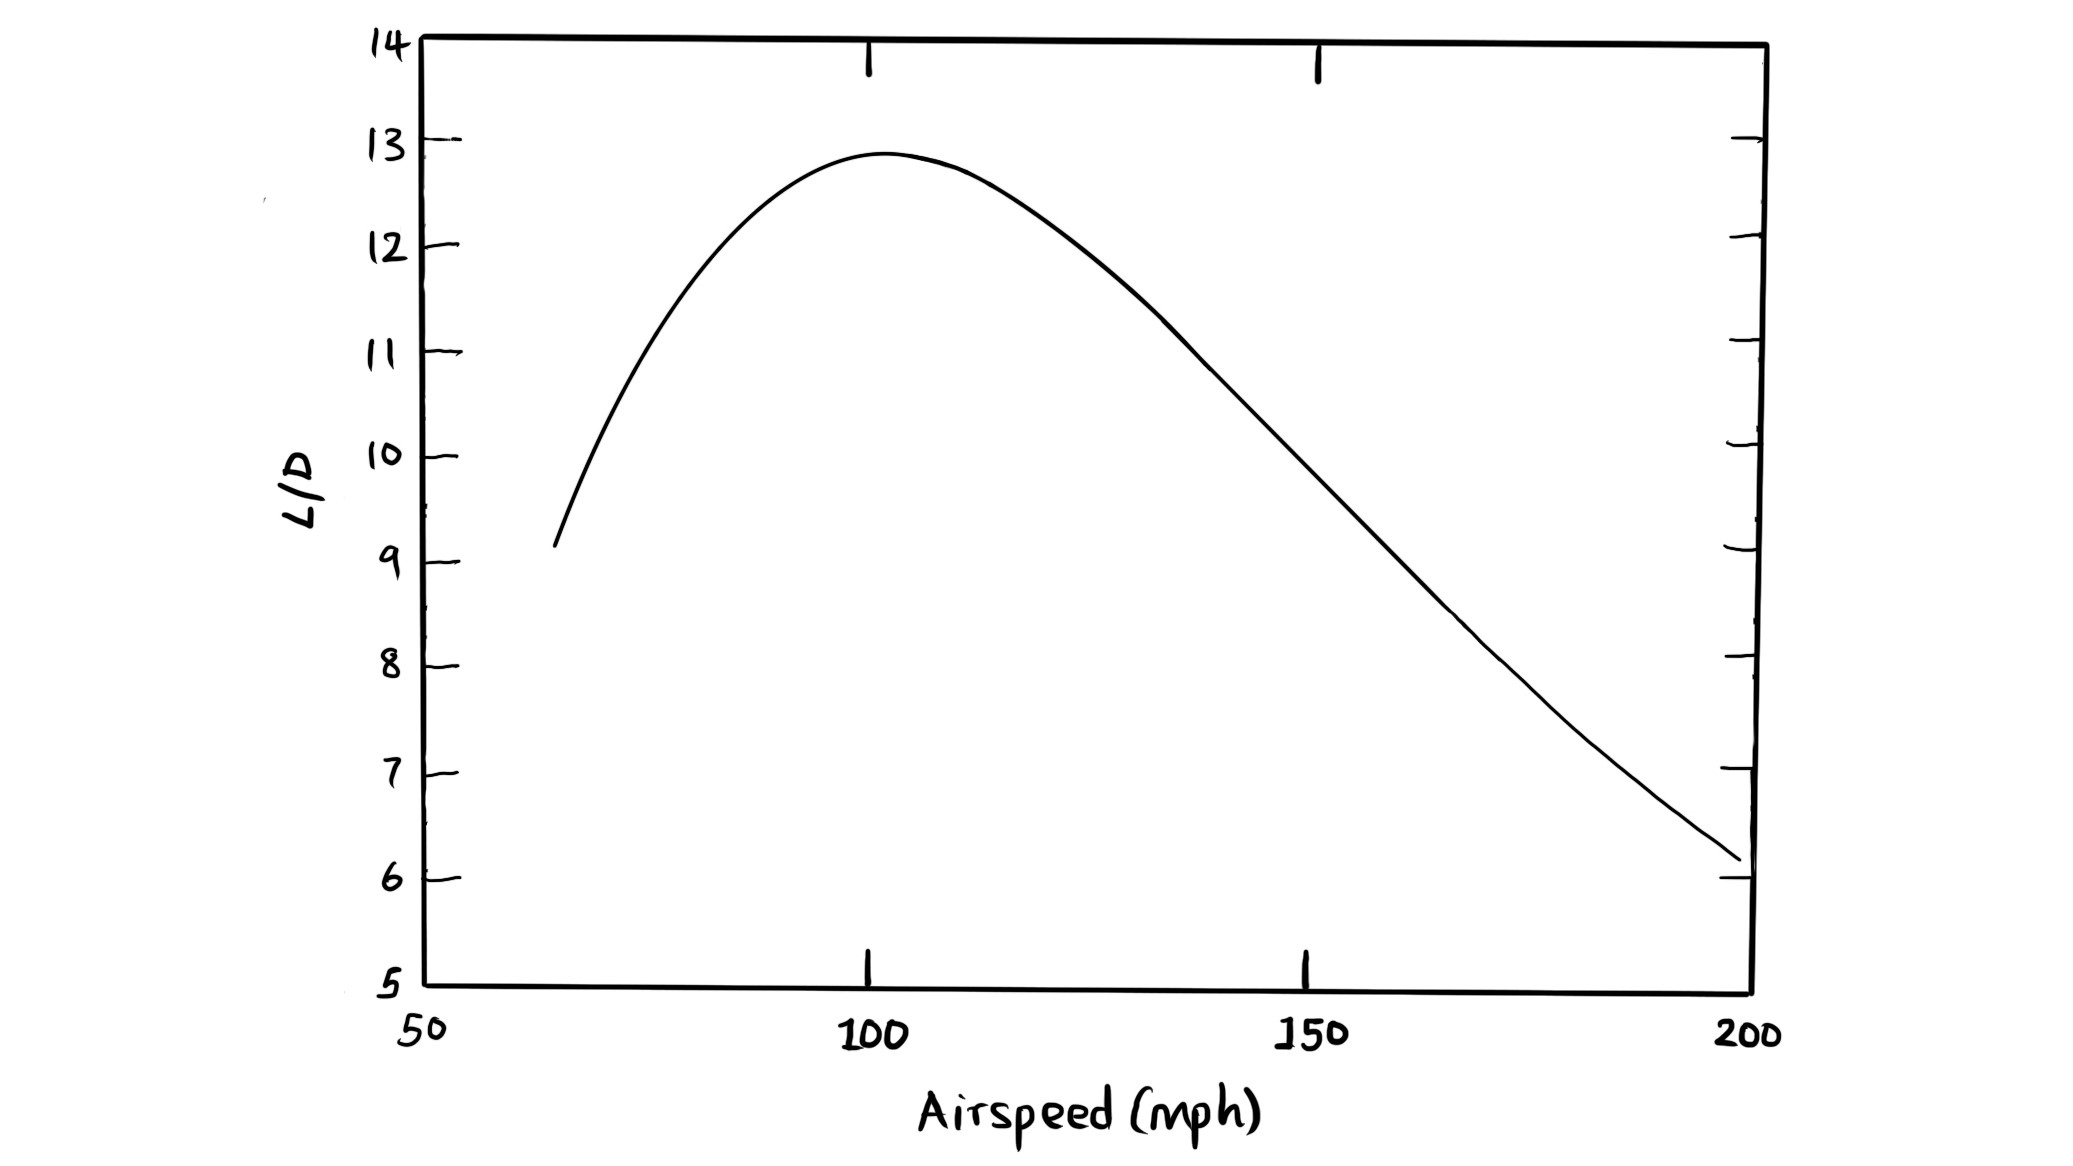
\includegraphics[scale=0.3]{plot_LD}
\centering
\caption{Typical variation of L/D ratio vs Airspeed at sea level}
\label{LDRvsV}
\end{figure}

When the thrust required is plotted versus airspeed, for a typical general aviation aircraft, it looks as shown in figure \ref{TRvsV}.
\begin{figure}[H]
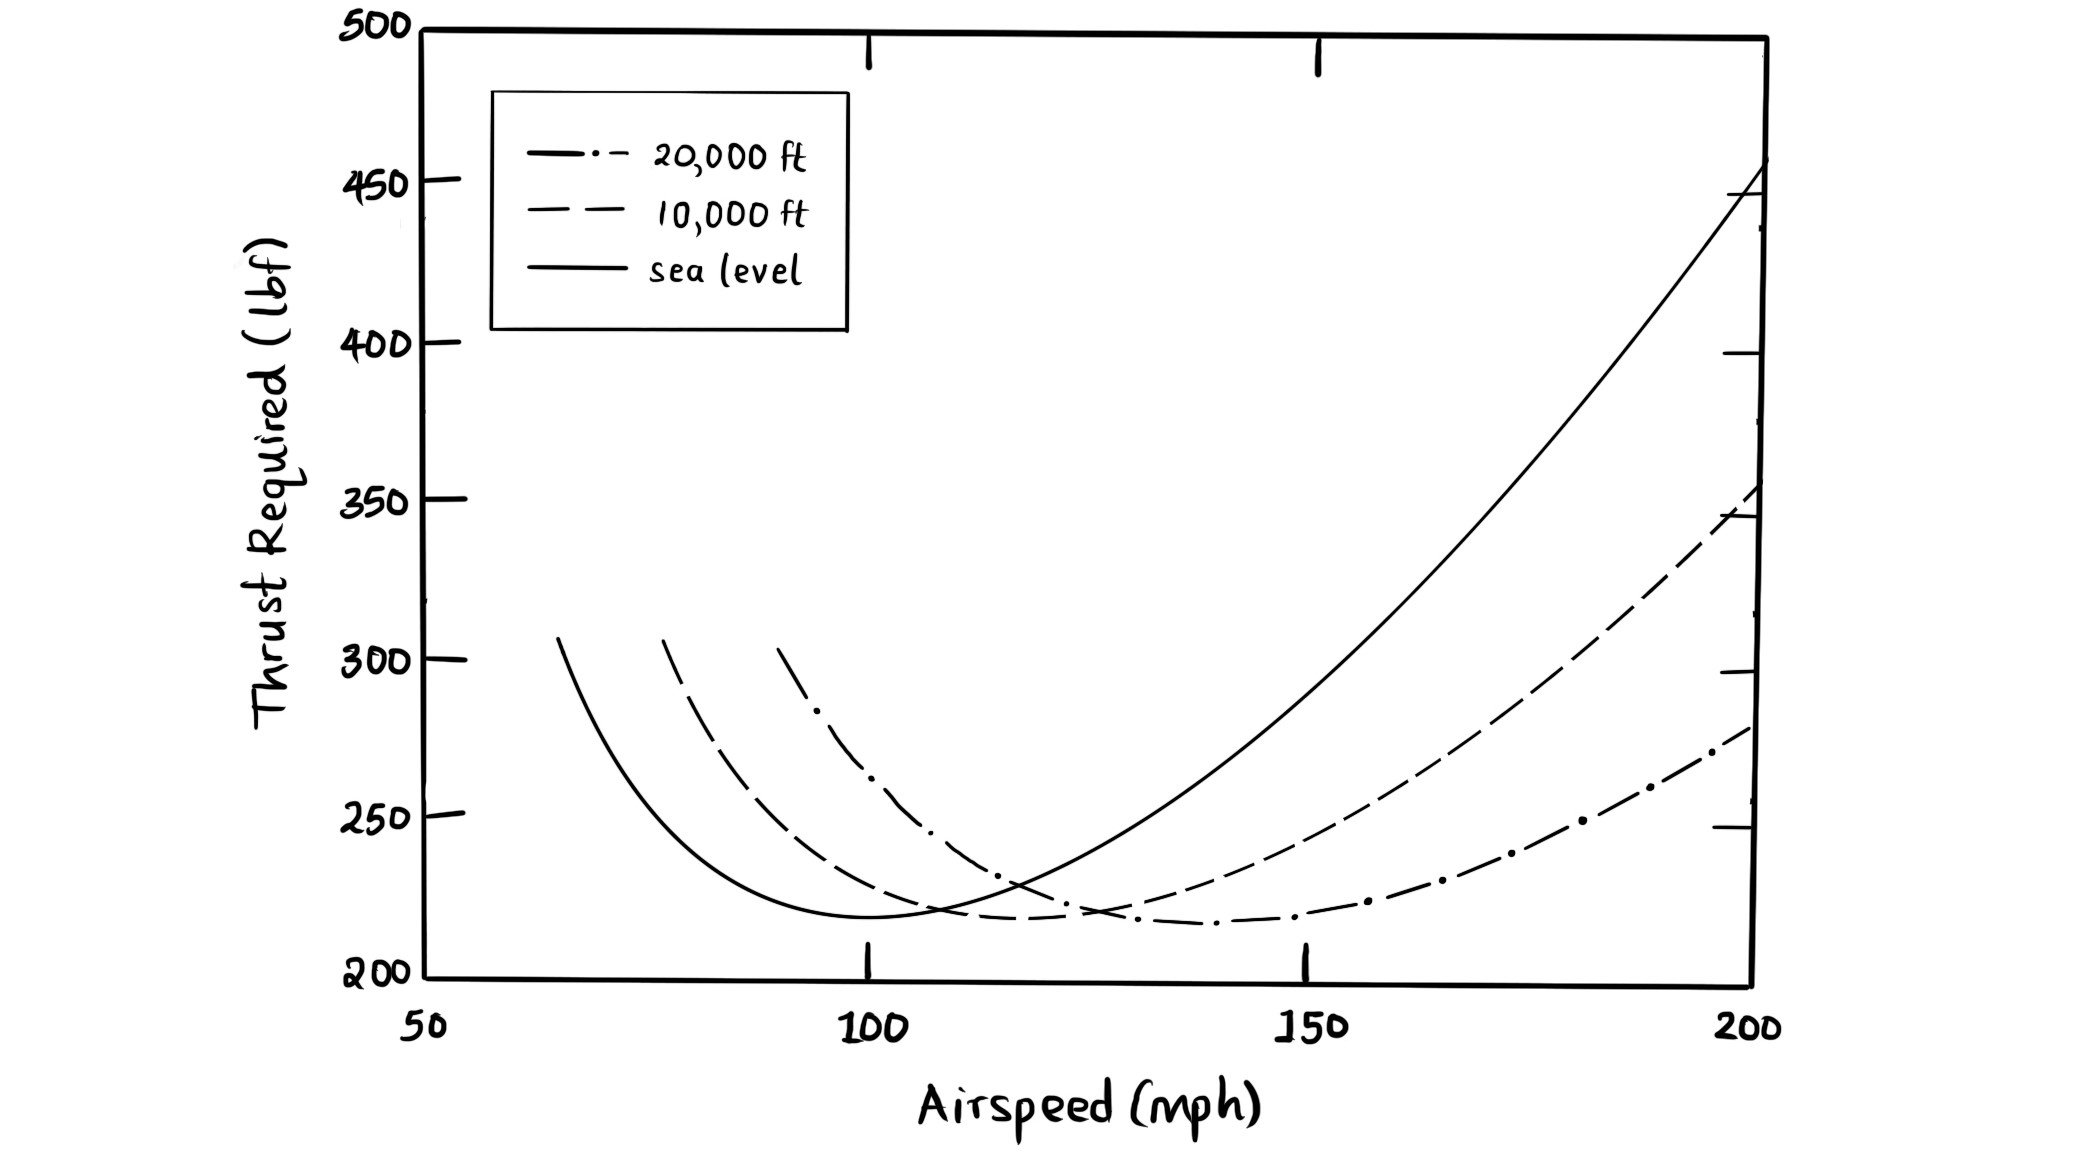
\includegraphics[scale=0.3]{plot_TR}
\centering
\caption{Typical variation of Thrust Required vs Airspeed}
\label{TRvsV}
\end{figure}

From equation \ref{thrust1}, we can obtain the optimum thrust angle, i.e. the value of $\alpha_T$ which minimizes the thrust required. This is done by differentiating the equation with respect to $\alpha_T$ and equating the result to zero. Thus, we get
\begin{equation}
\boxed{
\alpha_T=tan^{-1}(D/L).
}
\label{alphaT1}
\end{equation}

For conventional airplanes, in most cases, both $\alpha_T$ and $(D/L)$ are small values. Thus, we can safely use the following approximations for preliminary performance calculations
\begin{align*}
cos\alpha_T&\approx 1\\
sin\alpha_T&\approx \alpha_T\\
(D/L)sin\alpha_T&\approx \alpha_T^2\approx 0
\end{align*}.
This is termed \textit{small-thrust-angle approximation}. Applying this, expressions for Thrust required and Lift become simplified and equation \ref{thrust1} reduces to
\begin{equation}
T_R=D,
\end{equation}
\begin{equation}
L=W,
\end{equation}
\begin{equation}
T_R=\frac{W}{L/D}.
\label{thrust2}
\end{equation}

\paragraph{Power required}
The power required can be obtained by multiplying the thrust required by the airspeed and cosine of the thrust angle.
\begin{equation}
\boxed{
P_R=T_RVcos\alpha_T=DV,
}
\label{power1}
\end{equation}
where $P_R$ is the power required for steady level flight. Figure \ref{PR} shows a typical plot of power required versus airspeed for a general aviation aircraft.
\begin{figure}[H]
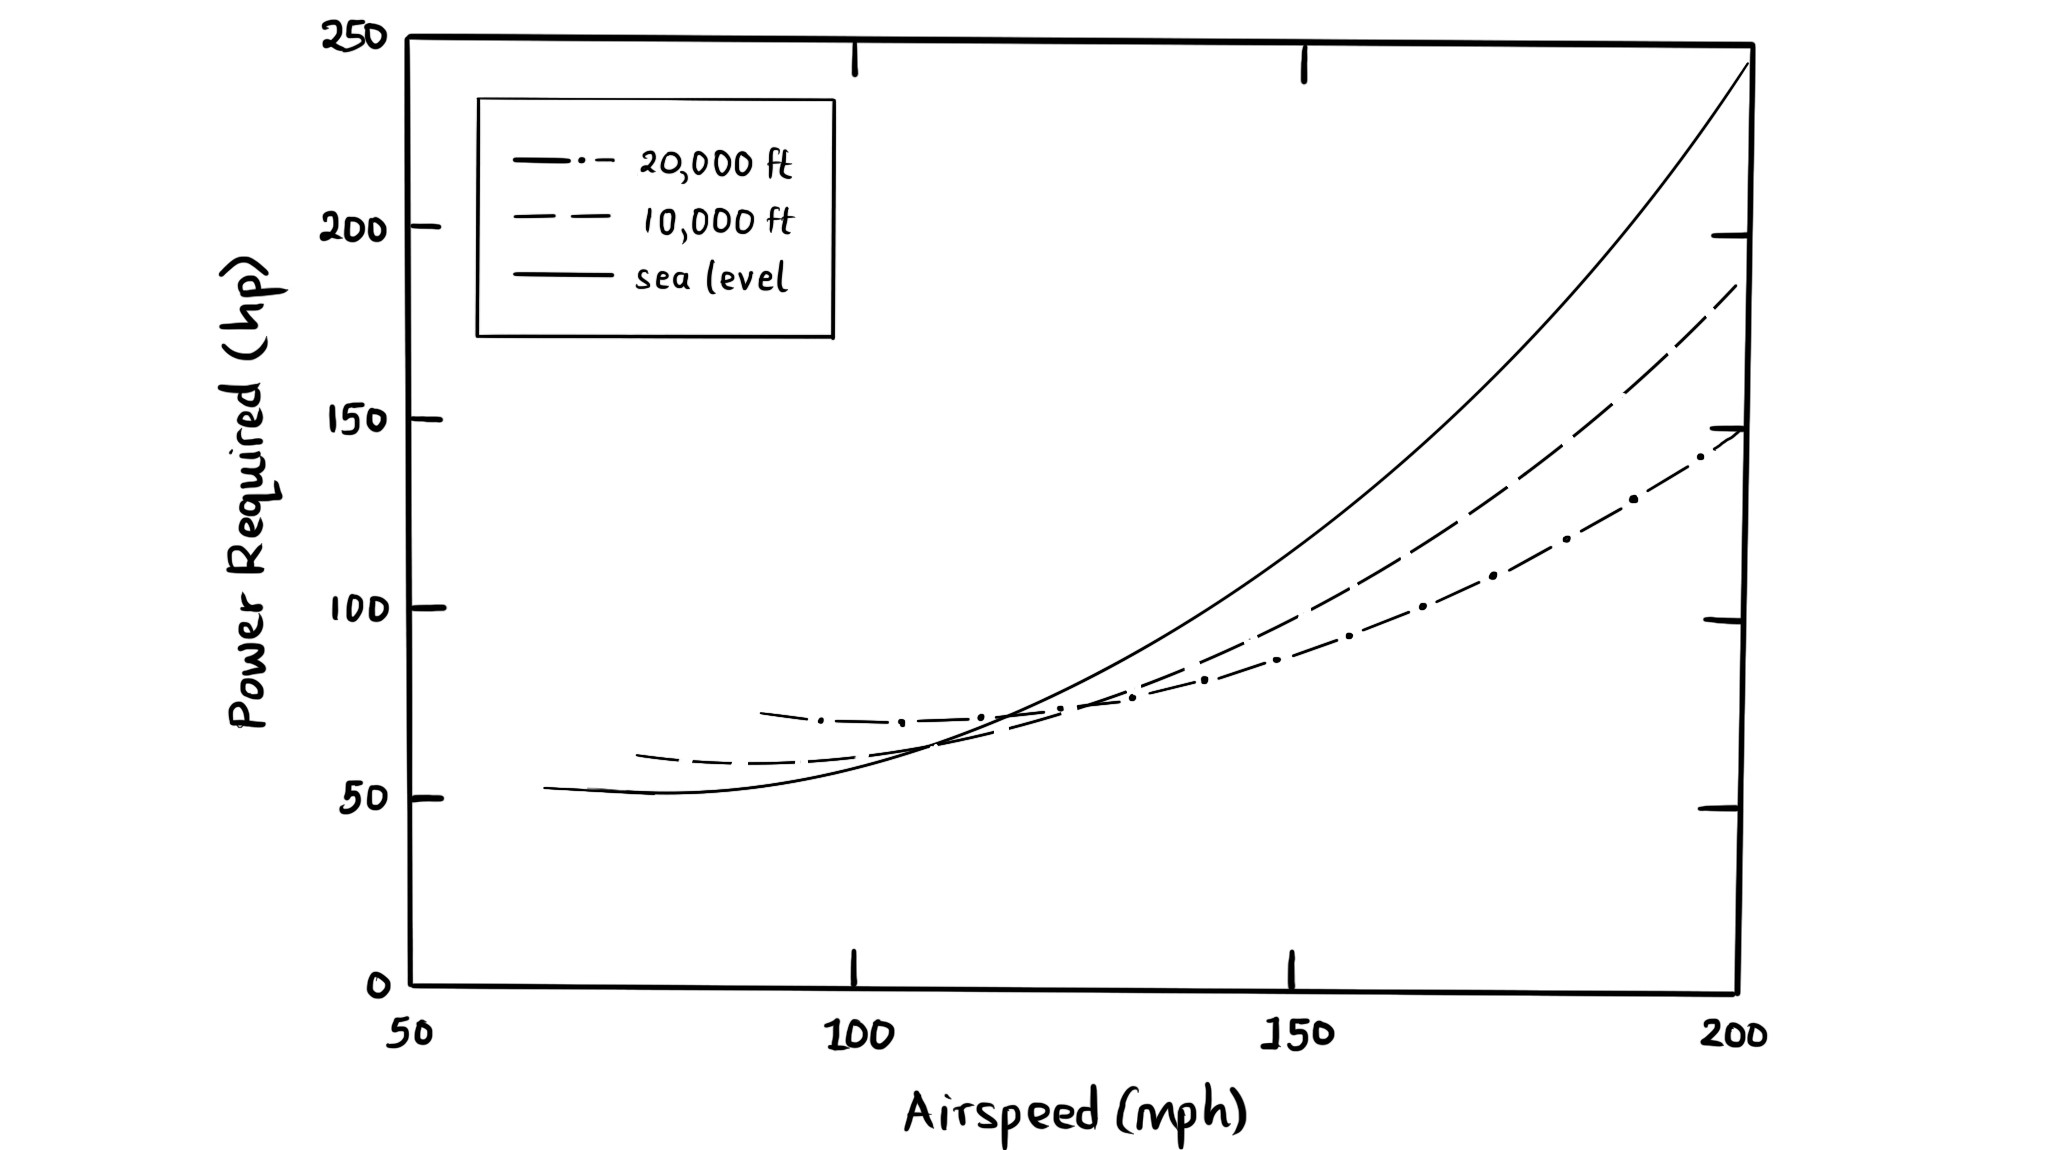
\includegraphics[scale=0.3]{plot_PR}
\centering
\caption{Typical variation of Power Required vs Airspeed}
\label{PR}
\end{figure}

\paragraph{Rate of Climb}
The rate of climb is a function of the aerodynamic design, weight of the aircraft and the power available from the engines. To find out the \textit{steady} rate of climb, consider an airplane in unaccelerated climbing flight as shown in figure \ref{forces-climb}. $T_A$ denotes the thrust available, and $\gamma$ is the angle between the flight path relative to the ambient air and the horizontal.
\begin{figure}[H]
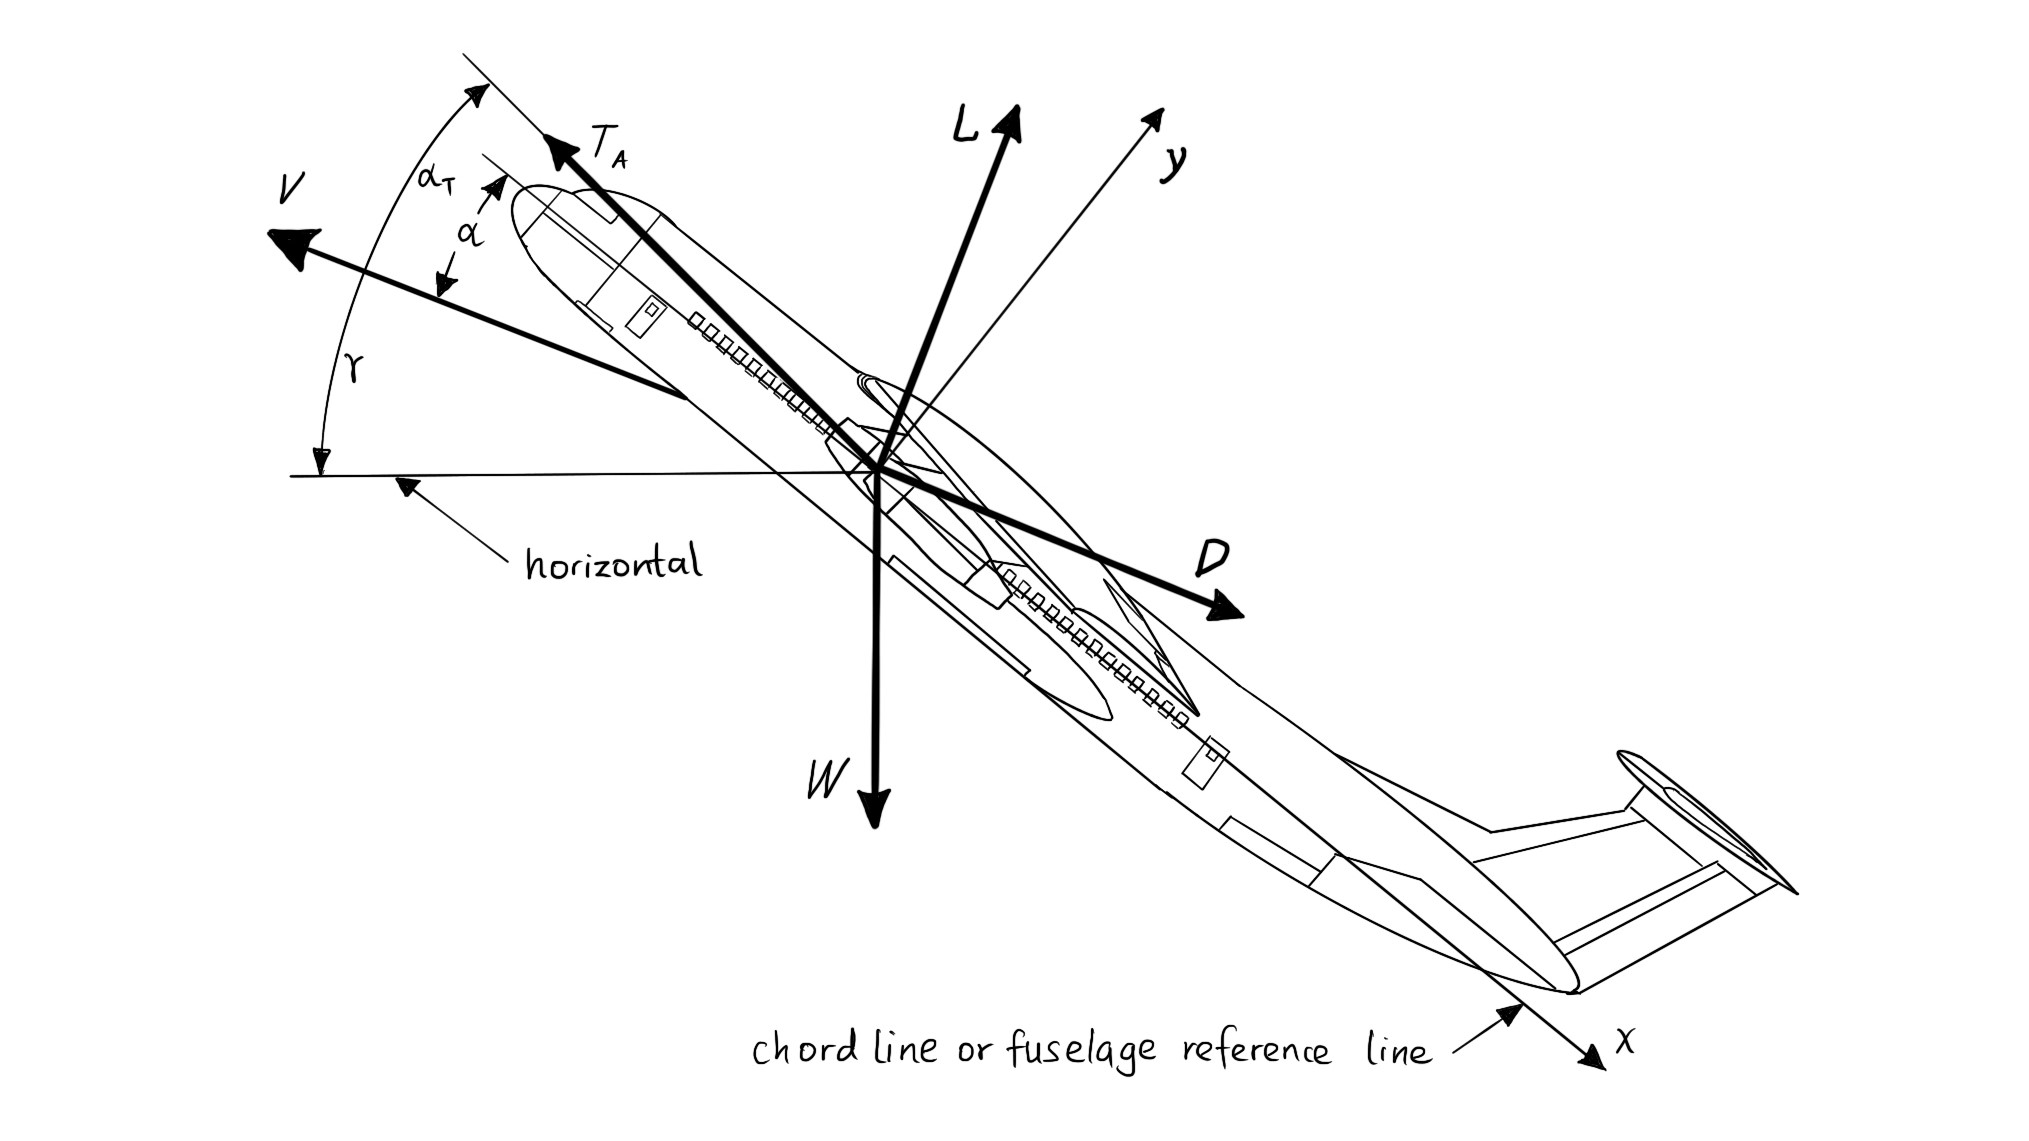
\includegraphics[scale=0.4]{forces_climb}
\centering
\caption{Forces acting on an aircraft in climb}
\label{forces-climb}
\end{figure}

The drag must be equal to the component of thrust parallel to the flight path minus the component of weight aligned with the flight path
\begin{equation}
D=T_Acos\alpha_T-Wsin\gamma.
\label{drag-climb}
\end{equation}

The lift can be computed as the weight component perpendicular to the flight path minus the thrust component normal to the flight path
\begin{equation}
L=Wcos\gamma-T_Asin\alpha_T.
\end{equation}

Applying these expressions to equation \ref{drag2} and definition of lift coefficient, we can obtain the \textit{general formulation for steady climbing flight}
\begin{equation}
\frac{1}{2}\rho V^2S_w\left(C_{D_0}+C_{{D_0},L}C_L+\frac{C_L^2}{\pi eR_A}\right)=T_Acos\alpha_T-Wsin\gamma.
\end{equation}

\begin{equation}
\frac{1}{2}\rho V^2S_wC_L=Wcos\gamma-T_Asin\alpha_T.
\end{equation}

The rate of climb, $V_c$, is basically the vertical component of the airplane's velocity, i.e. airspeed multiplied by the sine of flight path angle
\[
V_c=Vsin\gamma.
\]

From equation \ref{drag-climb}, we can obtain
\begin{equation}
sin\gamma=\frac{T_Acos\alpha_T-D}{W}.
\end{equation}

Thus, rate of climb can be written as
\begin{equation}
V_c=\frac{VT_Acos\alpha_T-VD}{W}.
\end{equation}

Now, since the climb angle is mostly small, we can use the value of drag for level flight here as an approximate estimate. Substituting the expression we discussed for level flight drag, the rate of climb can be written as
\begin{equation}
V_c=\frac{VT_Acos\alpha_T-VT_Rcos\alpha_T}{W}.
\end{equation}
Further, the product of airspeed with thrust available and cosine of the thrust angle, is the dot product of the thrust vector with the velocity vector which is the definition of Power available, $P_A$. Also, the airspeed multiplied by thrust required for level flight and cosine of the thrust angle is the definition of power required for level flight, $P_R$. Thus, the rate of climb can be further written as
\begin{equation}
\boxed{
V_c=\frac{P_A-P_R}{W}.
}
\label{roc-final}
\end{equation}

Figure \ref{ROC} shows a typical plot of Rate of Climb versus Airspeed for a general aviation aircraft at sea level for different throttle settings, $\tau$ defined as a fraction of the full-throttle power available.
\begin{figure}
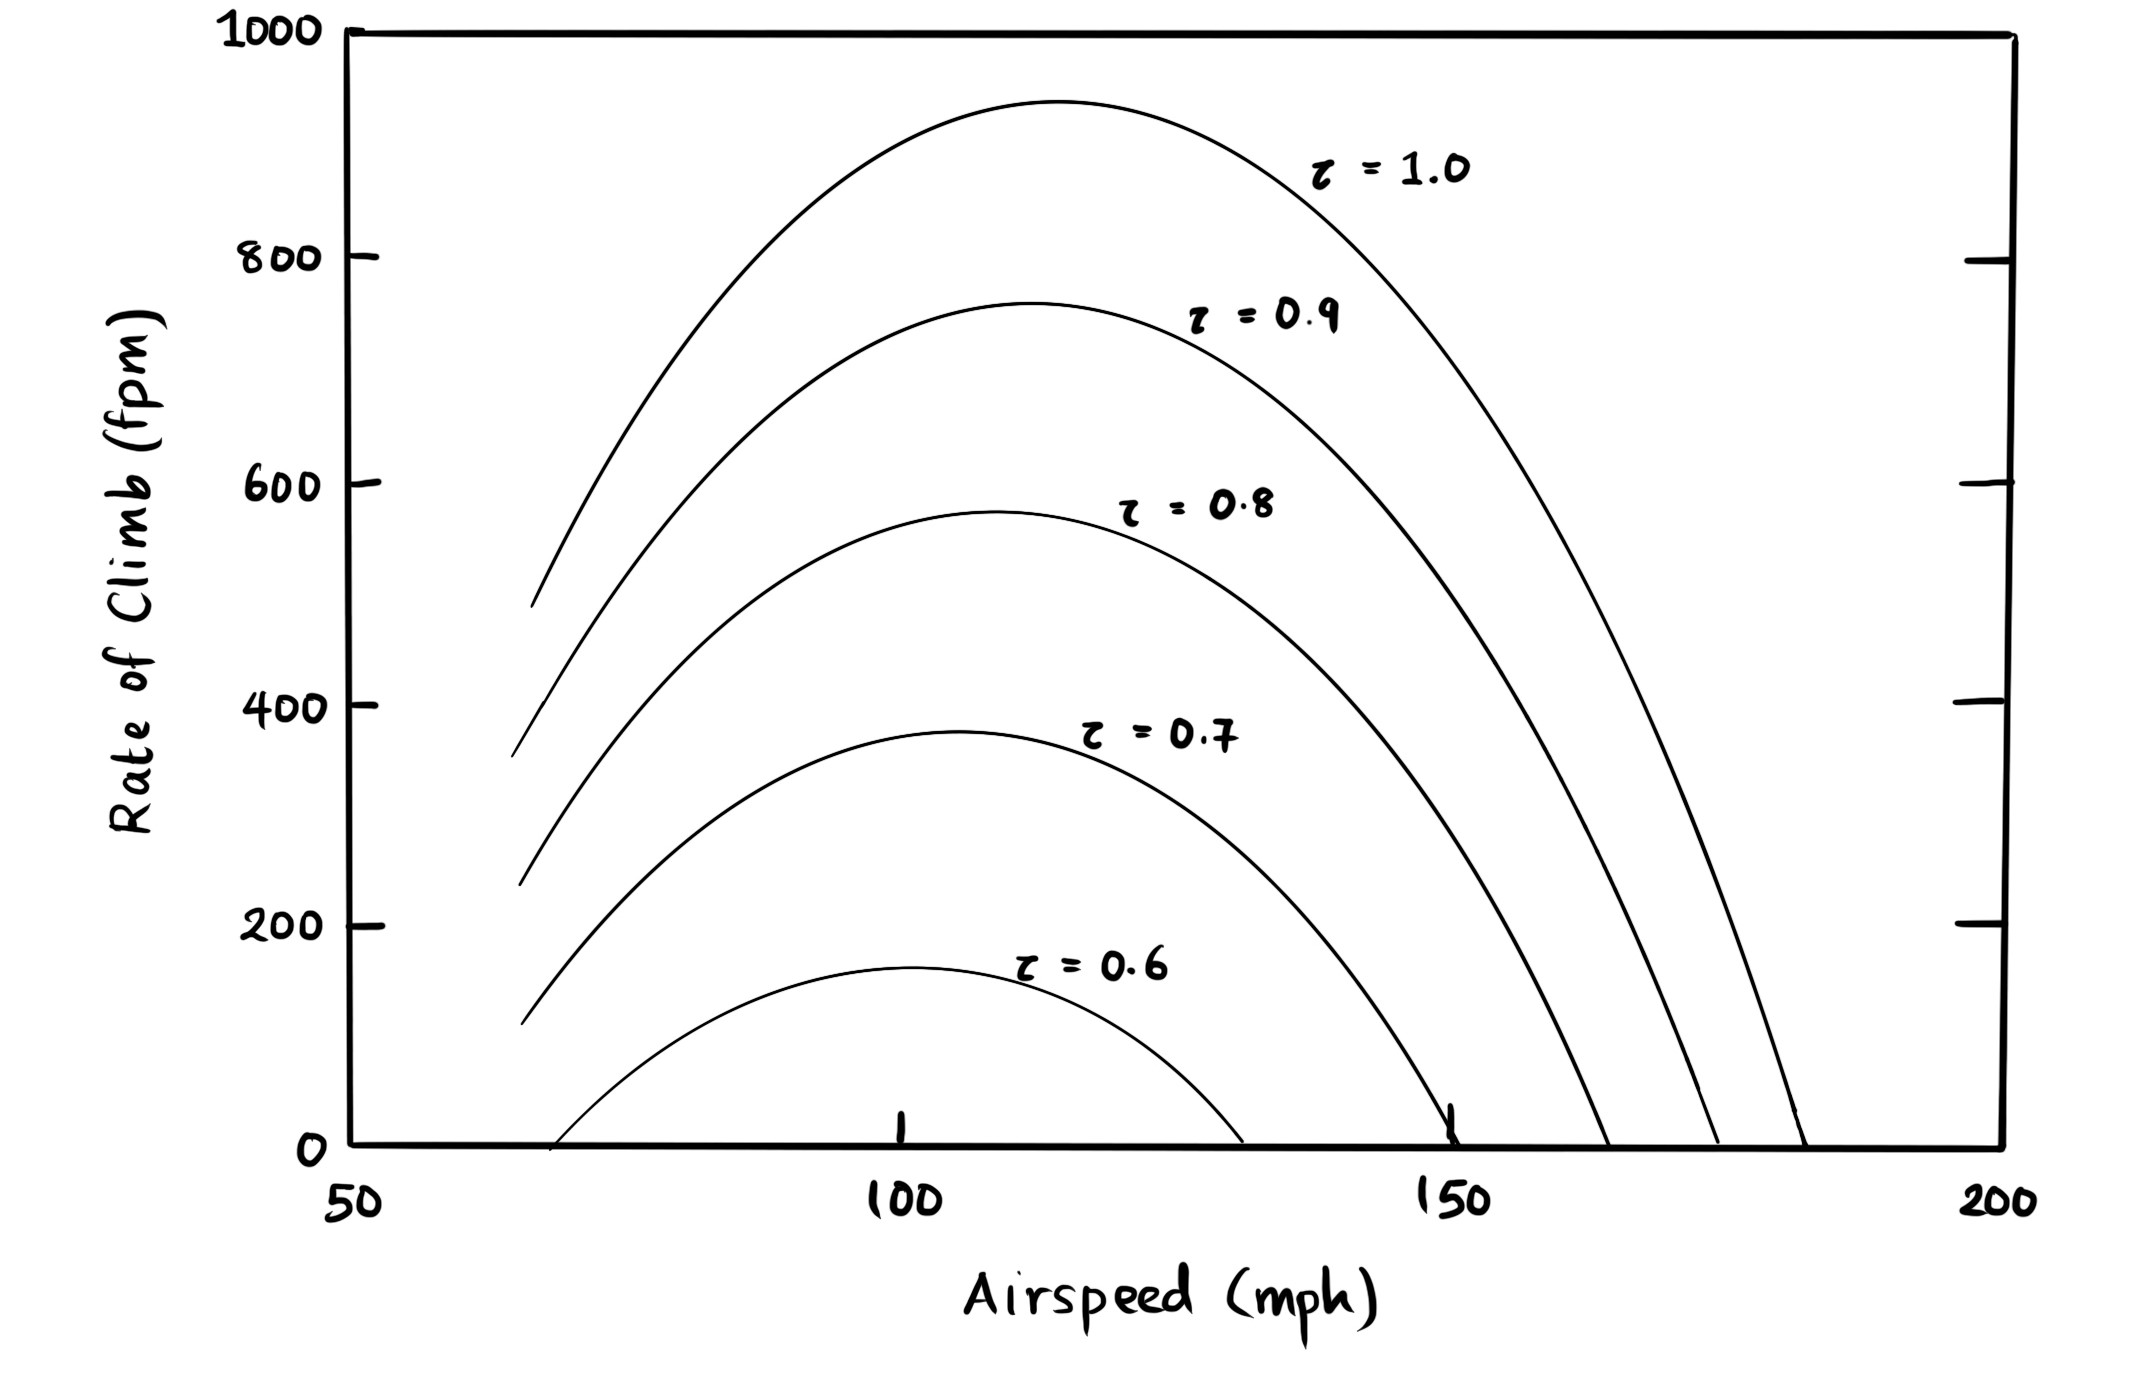
\includegraphics[scale=0.3]{plot_ROC}
\centering
\caption{Typical variation of Rate of Climb vs Airspeed at sea level}
\label{ROC}
\end{figure}

\paragraph{Fuel consumption}
Fuel consumption directly affects the endurance, defined as the total time an aircraft can fly on a given tank of fuel. To maximize endurance for a given aircraft and fuel capacity, we need to minimize fuel consumption per unit time. The power-specific fuel consumption for an engine, $q_P$, can be defined as the ratio between the weight of fuel consumption per unit time and the available power.
\begin{equation}
q_P=\frac{\dot Q}{P_A}.
\end{equation}

For steady level flight, the power available will be equal to the power required, $P_A=P_R$. Hence, we can find fuel consumption per unit time, represented by $q$ in the code, by simply multiplying $q_P$ and $P_R$
\begin{equation}
\boxed{
q=q_P . P_R.
}
\label{fuelc}
\end{equation}

The fuel consumption varies with airspeed for steady level flight as shown in figure \ref{FCvsV}.
\begin{figure}[H]
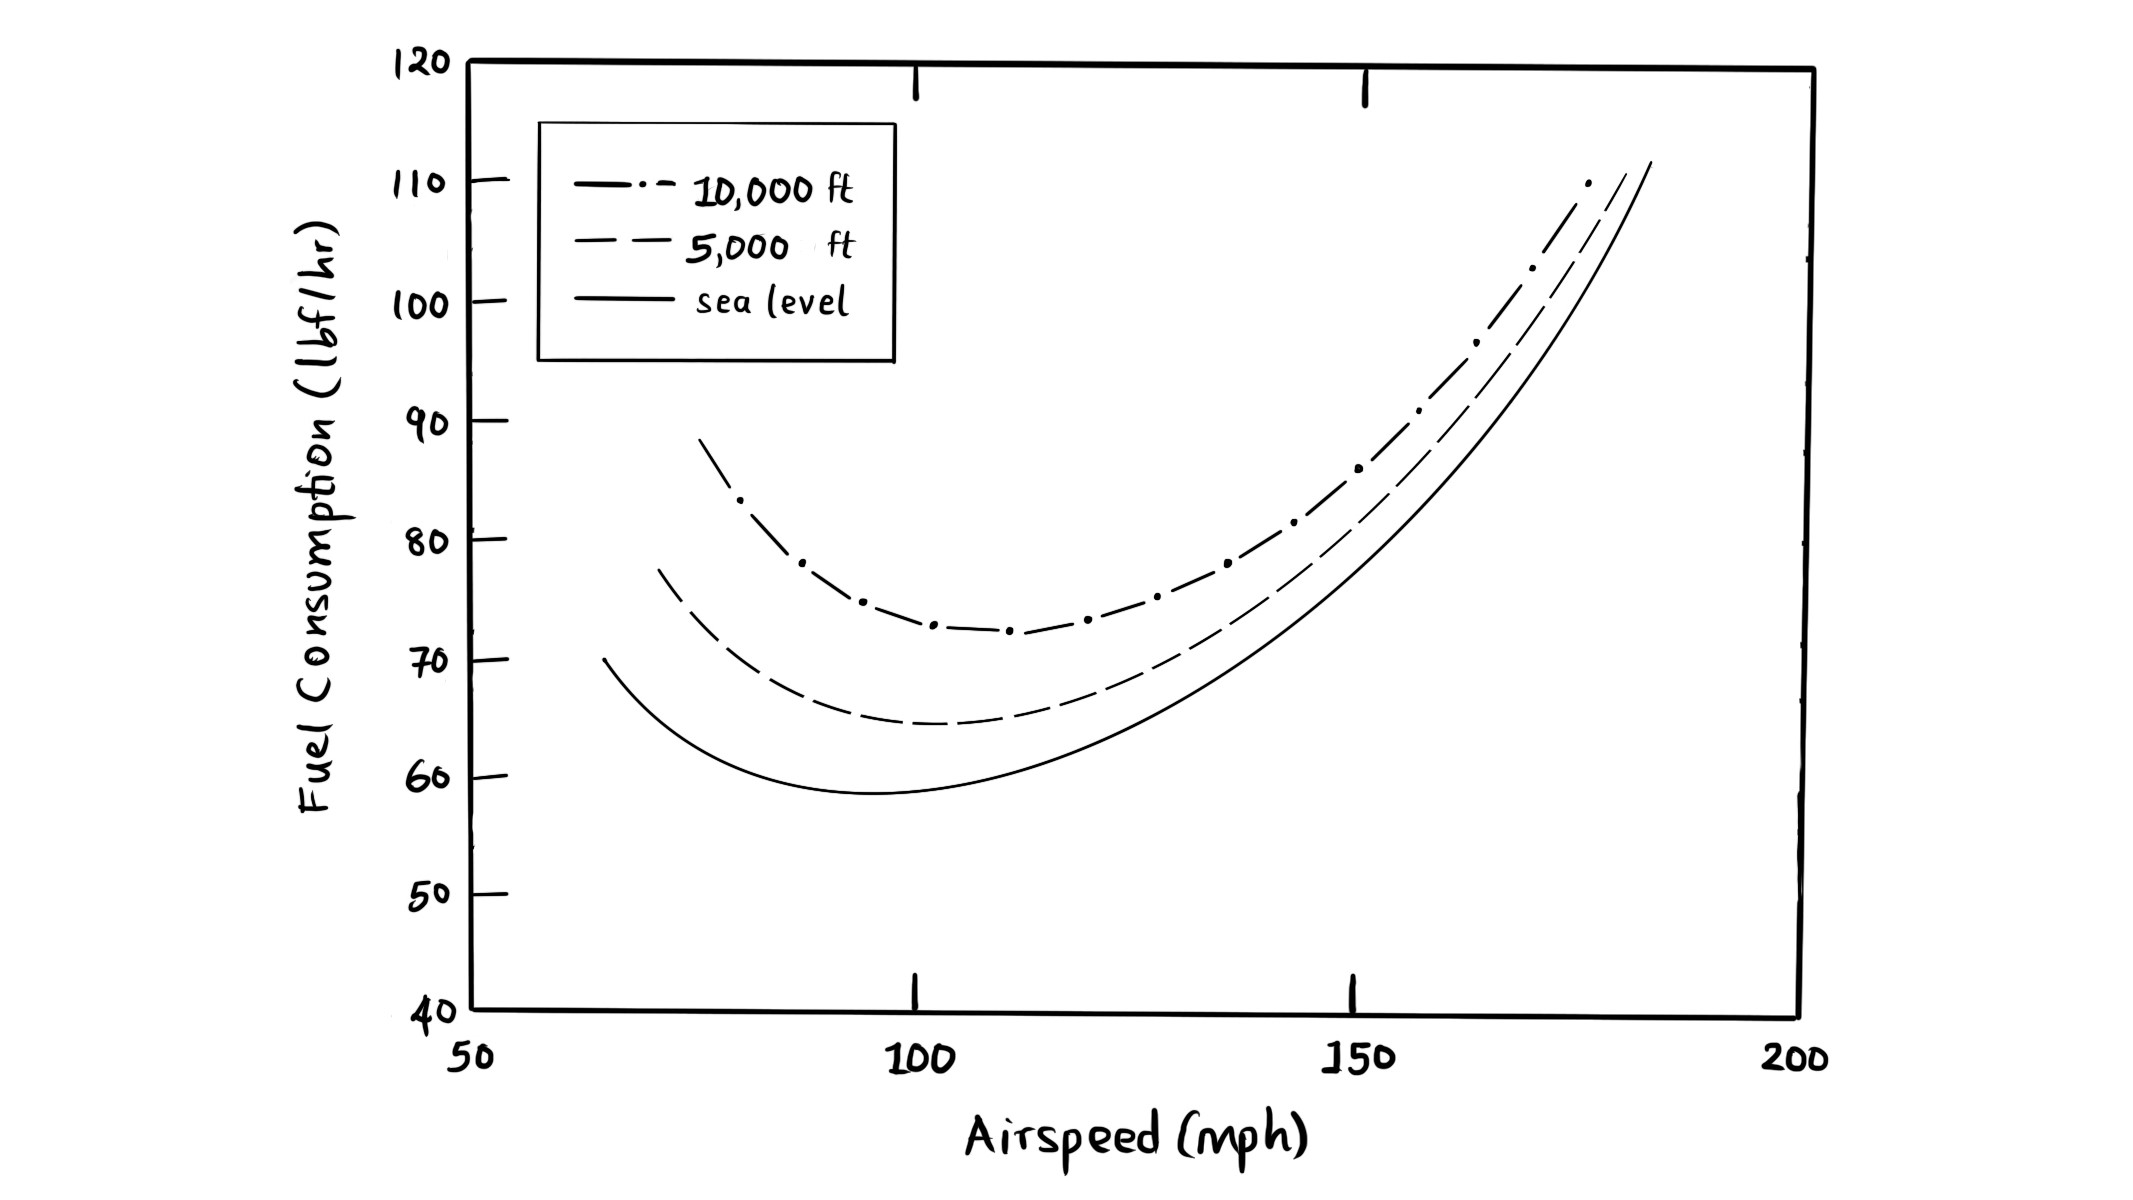
\includegraphics[scale=0.3]{plot_fuel}
\centering
\caption{Typical variation of Fuel Consumption vs Airspeed for steady level flight}
\label{FCvsV}
\end{figure}

\paragraph{Specific range}
Range is defined as the total distance an aircraft can fly for a given tank of fuel. Range can also be maximized by minimizing fuel consumption. It is helpful to define Specific range as the fuel consumed per unit distance. 
\begin{equation}
\boxed{
r_s = \frac{q}{v}.
}
\label{sr}
\end{equation}

A typical plot of variation of Specific range with airspeed is shown in the figure \ref{SRvsV}.
\begin{figure}[H]
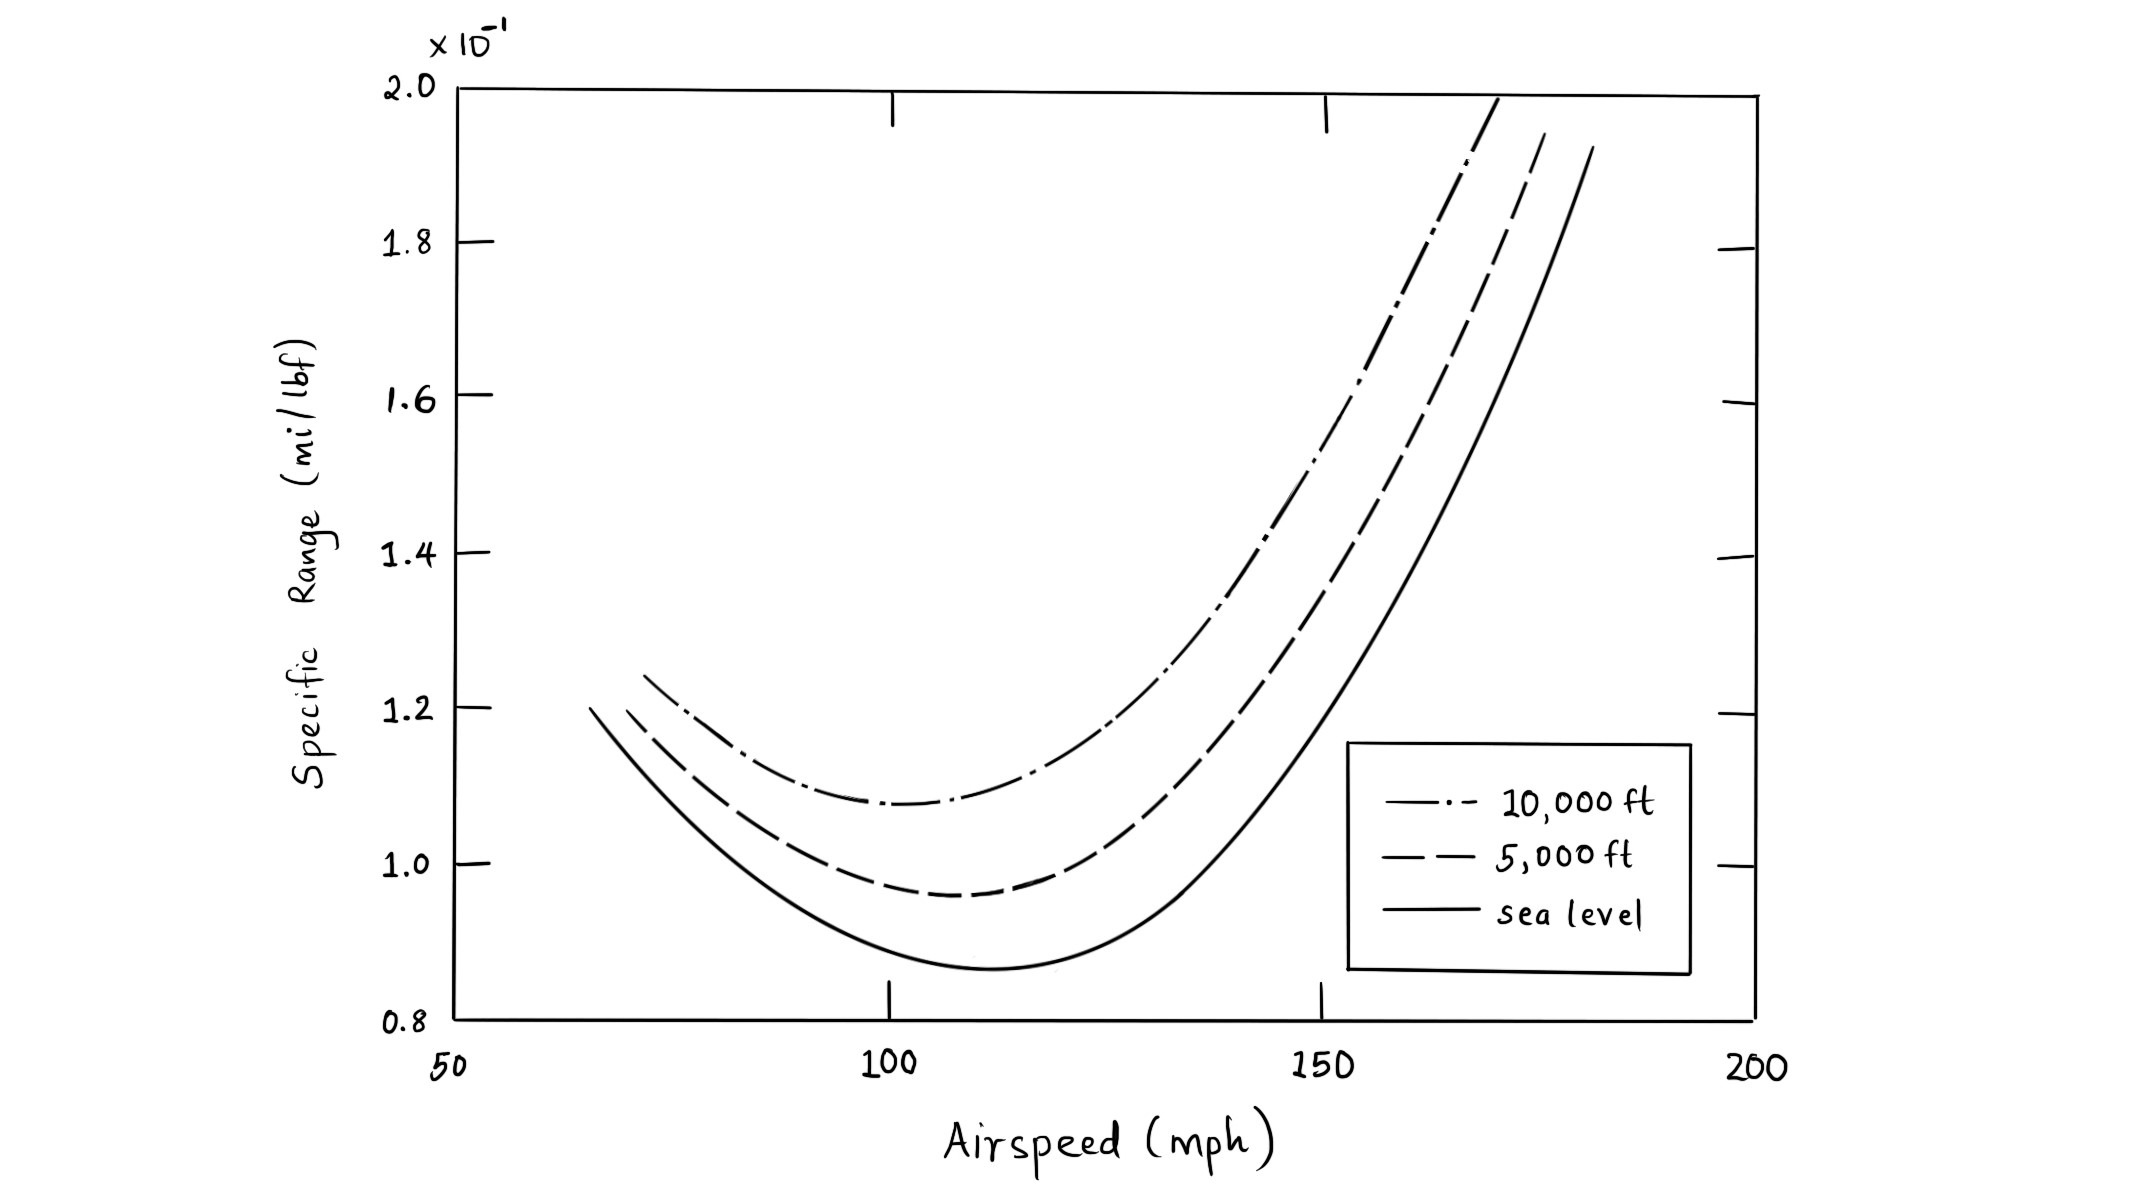
\includegraphics[scale=0.3]{plot_range}
\centering
\caption{Typical variation of Specific Range vs Airspeed at sea level}
\label{SRvsV}
\end{figure}

\paragraph{Stall speed}
The minimum airspeed at which the airplane can fly is termed the stall speed. The level flight stall speed is an important parameter and can be obtained as follows. Consider the expression for $C_L$ applying the small-thrust-angle approximation
\begin{equation}
C_L=\frac{W}{\frac{1}{2}\rho V^2S_w}.
\end{equation}

Solving for the expression for airspeed
\begin{equation}
V=\sqrt{\frac{2(W/S_w)}{\rho C_L}}.
\end{equation}

It can be seen that the value of velocity will be minimum when $C_L$ is at the maximum value. Therefore
\begin{equation}
\boxed{
V_{min}=\sqrt{\frac{2}{C_{L_{max}}}}\sqrt{\frac{(W/S_w)}{\rho}}.
}
\label{vmin}
\end{equation}


\subsubsection{Static stability}
\paragraph{Static margin}
Similar to the aerodynamic center of an airfoil, the whole aircraft has a point about which the total pitching moment is independent of the angle of attack. This point is termed \textit{stick-fixed neutral point} as the airplane will be neutrally stable in pitch if the center of gravity is located at this point. For an aircraft to be statically stable, it can be proven that the center of gravity must be forward of the stick-fixed neutral point. The distance of the CG from the neutral point, expressed as a fraction of the mean chord length, is termed \textit{stick-fixed static margin}. The expression is given in the equation \ref{lnp}.
\begin{figure}[H]
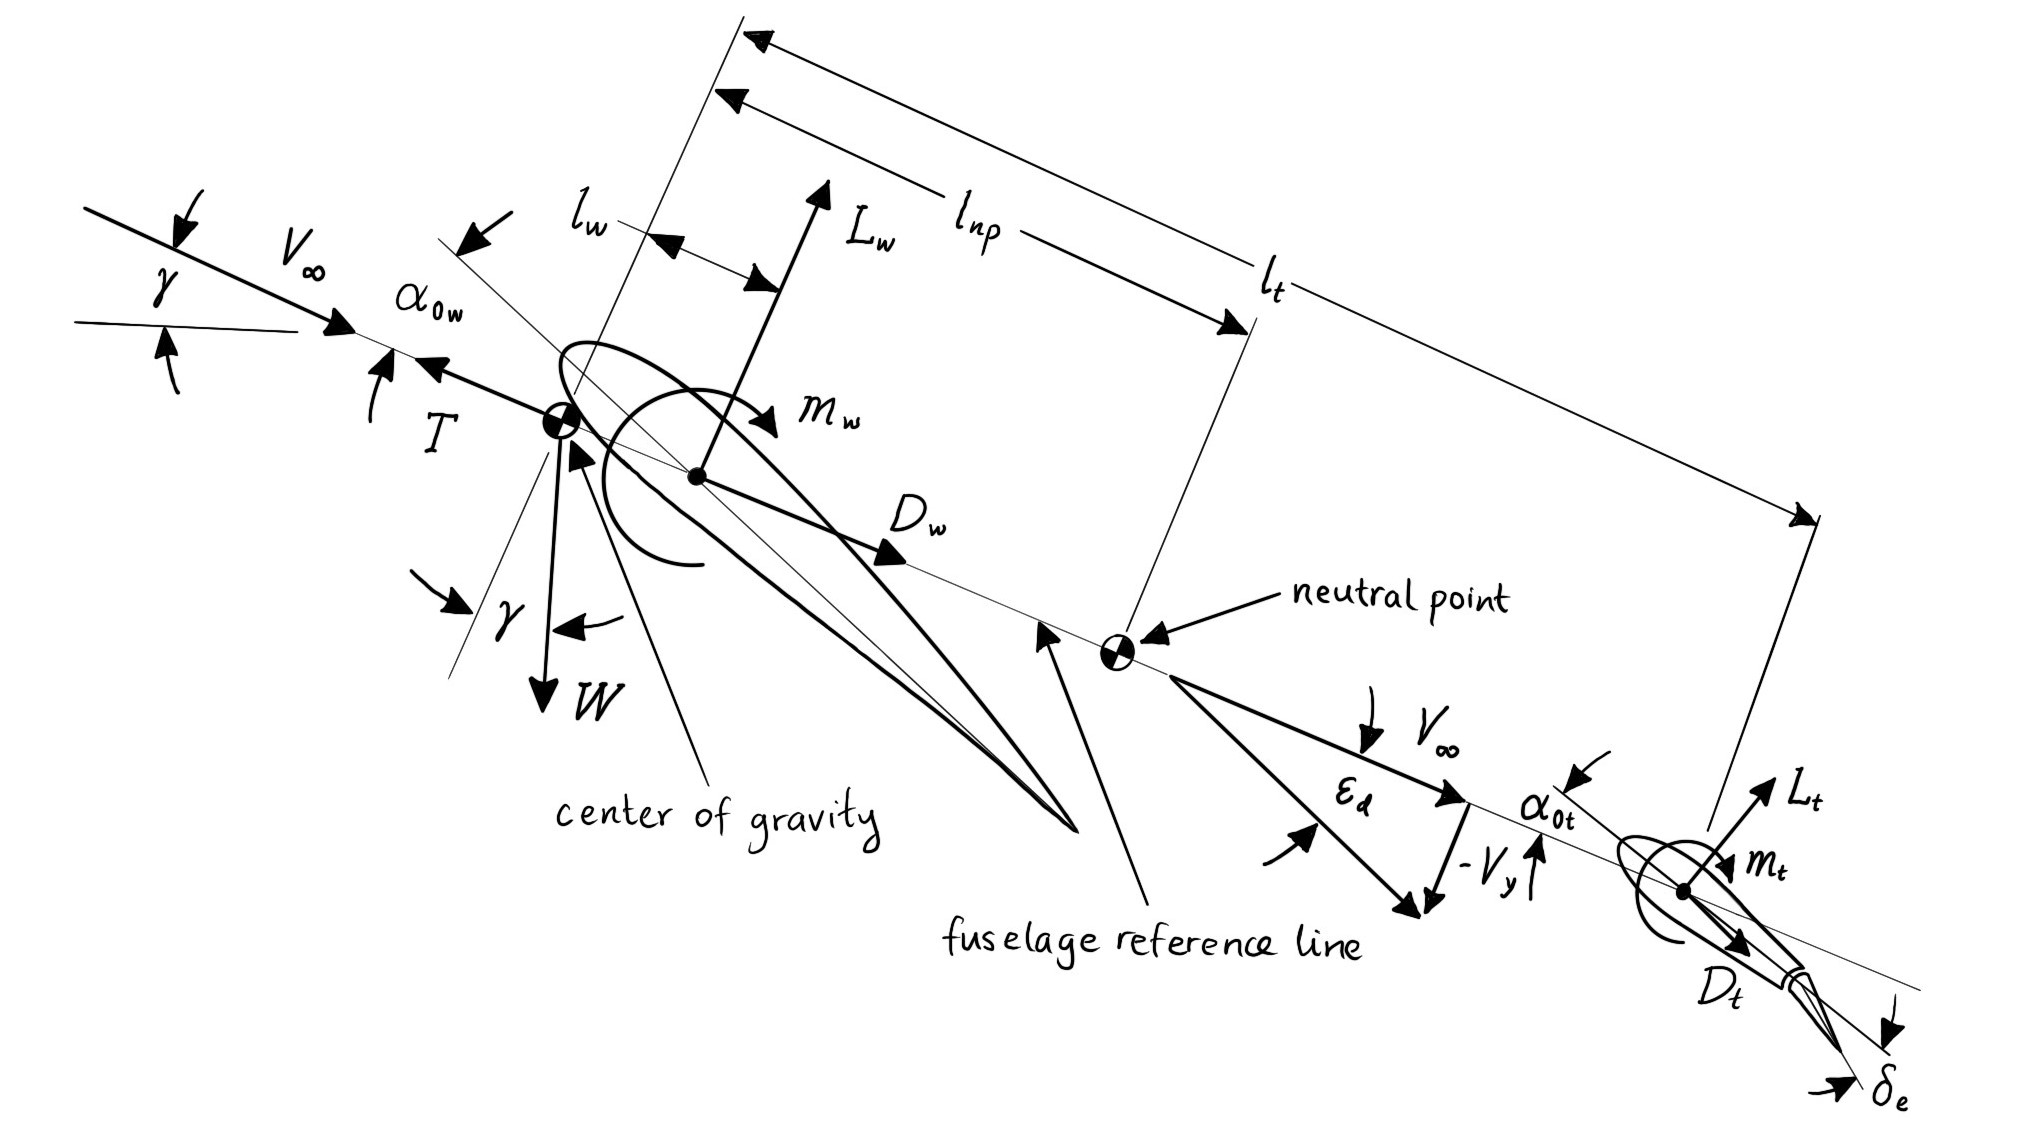
\includegraphics[scale=0.35]{st_margin}
\centering
\caption{Understanding the location of the stick-fixed neutral point}
\label{sm1}
\end{figure}
\begin{equation}
\boxed{
\frac{l_{np}}{\bar c_w}=\frac{l_wC_{L_w,\alpha}+\frac{S_tl_t}{S_w}\eta_tC_{L_t,\alpha}(1-\varepsilon_{d,\alpha})}{\bar c_w\left[C_{L_w,\alpha}+\frac{S_t}{S_w}\eta_tC_{L_t,\alpha}(1-\varepsilon_{d,\alpha})\right]}.
}
\label{lnp}
\end{equation}

The variables seen here denote
\begin{align*}
l_{np}&=\text{Distance between the stick-fixed neutral point and the CG}\\
\bar c_w&=\text{Mean chord length of the wing}\\
l_w&=\text{Distance from CG to the aerodynamic center of the wing}\\
l_t&=\text{Distance from CG to the aerodynamic center of the tail}\\
C_{L_w,\alpha}&=\text{Lift slope for the main wing}\\
C_{L_t,\alpha}&=\text{Lift slope for the isolated tail}\\
S_w, S_t&=\text{Planform areas of the wing and tail respectively}\\
\eta_t&=\text{Tail efficiency(can vary between 0.8 and 1.2 but usually assumed to be 1)}\\
\varepsilon_{d,\alpha}&=\text{Change in the downwash angle with respect to the angle of attack}\\
\end{align*}.

\paragraph{Yaw Stability Derivative}
Static yaw stability, which is the ability to naturally produce a restorative yawing moment opposing any disturbance in yaw faced by the airplane, is provided by the vertical tail mainly. The general criterion for static yaw stability mathematically is given by
\begin{equation}
\frac{\partial C_n}{\partial\beta}\equiv C_{n,\beta} \textgreater 0.
\end{equation}
$C_{n,\beta}$ represents the \textit{yaw stability derivative} or \textit{yaw stiffness}. The contribution of the vertical tail to the yaw stability derivative, which we are interested here in this section, is given by the equation \ref{yawder}. The various terms involved in that expression can be understood better through the figure \ref{sideslip} which shows the various yawing moments experienced by an aircraft in sideslip.
\begin{figure}[H]
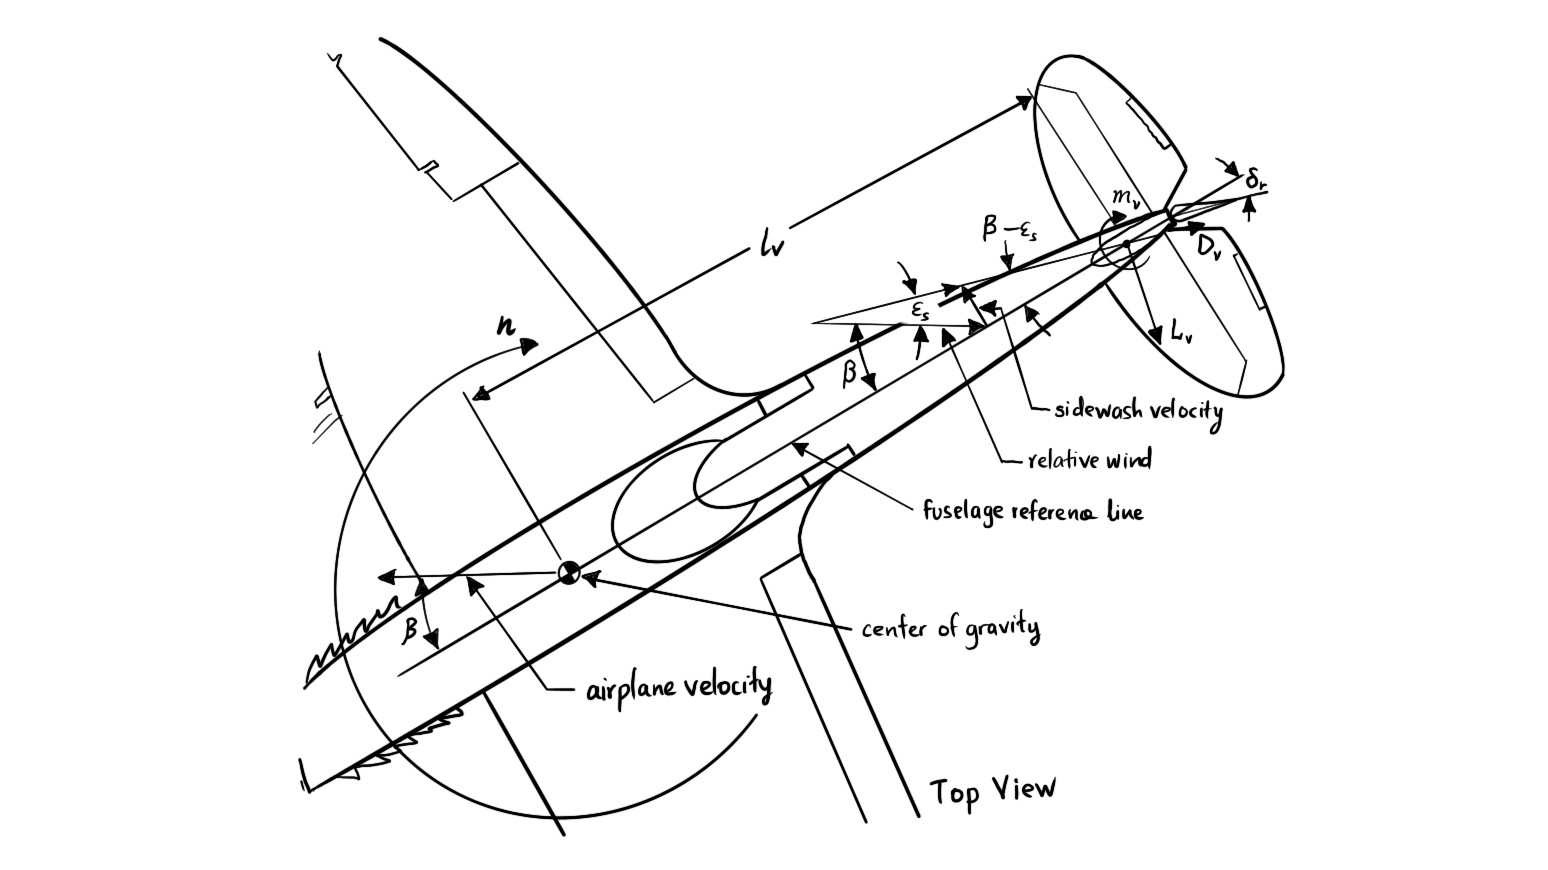
\includegraphics[scale=0.5]{yaw_der}
\centering
\caption{Top view of an airplane experiencing sideslip}
\label{sideslip}
\end{figure}

\vspace{10pt}

\begin{equation}
\boxed{
(\Delta C_{n,\beta})_v=\eta_v\frac{S_vl_v}{S_wb_w}C_{L_v,\alpha}(1-\varepsilon_{s,\beta})_v.
}
\label{yawder}
\end{equation}

The variables seen in this equation denote
\begin{align*}
\eta_v&=\text{Dynamic pressure ratio for the vertical tail}\\
l_v&=\text{Distance from CG to the aerodynamic center of the vertical tail}\\
b_w&=\text{Wingspan}\\
C_{L_v,\alpha}&=\text{Lift slope for the vertical tail}\\
S_w, S_v&=\text{Planform areas of the wing and vertical tail respectively}\\
\varepsilon_{s,\beta}&=\text{Sidewash gradient}\\
\varepsilon_{s,\beta}&\equiv\frac{\partial\varepsilon_s}{\partial\beta}\\
\varepsilon_s&=\text{Sidewash angle}\\
\beta&=\text{Sideslip angle}\\
\end{align*}.

\paragraph{Roll Stability Derivative}
If any disturbance in bank angle naturally produces a restoring rolling moment, the aircraft is said to have static roll stability. The general criterion for an aircraft to be statically stable in roll is given by
\begin{equation}
\frac{\partial C_l}{\partial\beta}\equiv C_{l,\beta} \textless 0,
\end{equation}
$C_{l,\beta}$ represents the \textit{roll stability derivative}. The contribution of the wing dihedral to the roll stability derivative is given by the expression \ref{clbg}. The effect can be understood better from the figure \ref{dihedral} which shows what happens to the rolling moment when an airplane is experiencing sideslip.
\begin{figure}[H]
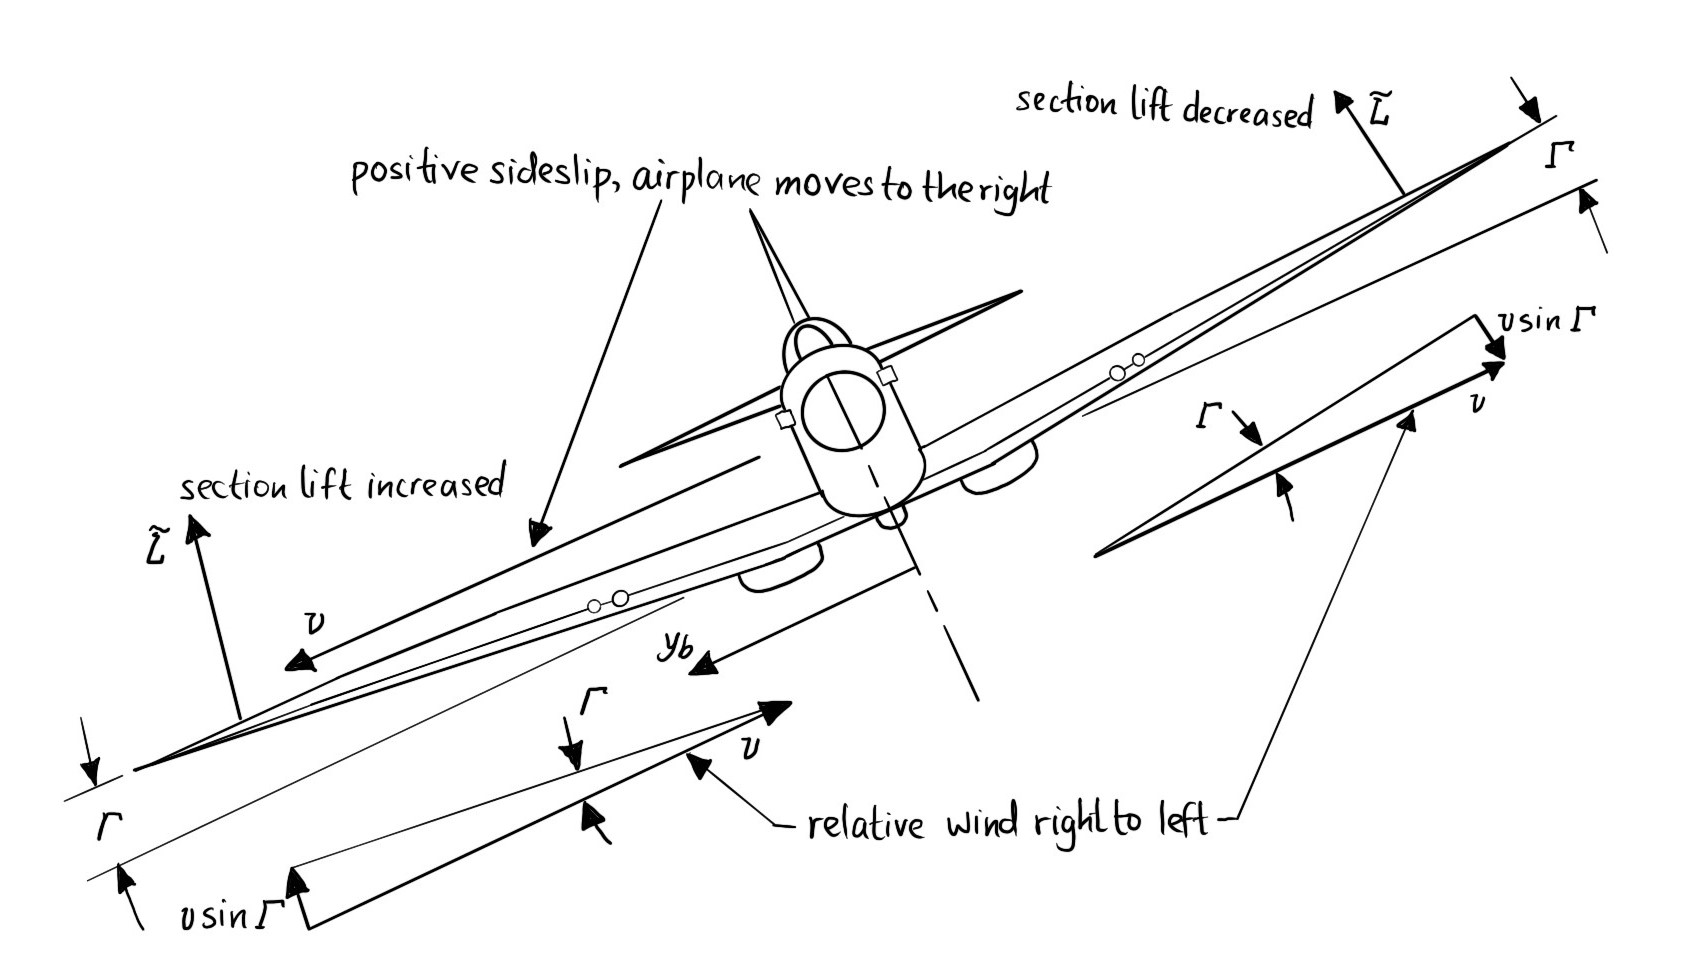
\includegraphics[scale=0.5]{roll_st}
\centering
\caption{Front view of airplane showing effect of dihedral}
\label{dihedral}
\end{figure}
\vspace{10pt}

\begin{equation}
\boxed{
(\Delta C_{l,\beta})_{\Gamma_w}=-\frac{2\Gamma}{3\pi}\kappa_lC_{L_w,\alpha}.
\label{clbg}
}
\end{equation}

The contribution of vertical tail to the roll stability derivative can be obtained by
\begin{equation}
\boxed{
(\Delta C_{l,\beta})_v=-\eta_v\frac{S_vh_v}{S_wb_w}(1-\varepsilon_{s,\beta})_vC_{L_v,\alpha}.
}
\label{clbv}
\end{equation}

A rough estimation of the contribution of the horizontal stabilizer to the rolling moment is calculated by the equation \ref{clbh}, where the positive sign is used when the stabilizer is mounted below the vertical tail and the negative sign is used when it is mounted above the vertical tail.
\begin{equation}
\boxed{
(\Delta C_{l,\beta})_h=\pm0.08\eta_v\frac{S_vb_h}{S_wb_w}(1-\varepsilon_{s,\beta})_vC_{L_v,\alpha}.
\label{clbh}
}
\end{equation}

The total roll derivative can be found by simply adding the individual contributions.

\subsection{The python code}
\lstset{inputpath=./performance/}

\subsubsection{Performance}

This code calculates the general performance parameters using the equations discussed in the theory above. There are a wide range of inputs needed including the environmental values, the aircraft parameters (Cessna 172 in this example), the engine parameters. The code snippet is included here, the variables defined are explained sufficiently in the comments.
\lstinputlisting[firstline=5,lastline=26,caption=Input values]{performance.py}

The function stall\_speeds is defined to calculate and print the stall speeds both with and without flaps using the corresponding $C_{L,max}$ value, using equation \ref{vmin}.
\lstinputlisting[firstline=32,lastline=44,caption=Stall speeds]{performance.py}

The lift\_to\_drag function is defined to find the Lift to drag ratio and optimize the thrust offset. We start out by assuming an initial value for L/D ratio as 5, as an input to find the initial $C_L$ value using equation \ref{cl1}, and then iterate using equation \ref{LDratio}. Then, the angle between the thrust vector and the direction of flight is calculated using equation \ref{alphaT1}.
\lstinputlisting[firstline=47,lastline=76,caption=L/D ratio]{performance.py}

The rest of the functions are straightforward applications of the concepts discussed above, specifically equations \ref{thrust2}, \ref{power1}, \ref{roc-final}, \ref{fuelc}, \ref{sr}, to calculate the corresponding parameters and plot the results.

\lstinputlisting[firstline=79,lastline=172,caption=Performance calculations]{performance.py}

\subsubsection{Static Stability}
This code deals with finding the values of \textit{static margin}, \textit{yaw derivative} and \textit{roll derivative} for a given aircraft. 
\lstinputlisting[firstline=3,lastline=23,caption=Input values]{static_stability.py}
Using equations \ref{lnp}, \ref{yawder}, \ref{clbg}, \ref{clbv}, \ref{clbh}, the required values are determined.
\lstinputlisting[firstline=26,lastline=68,caption=Input values]{static_stability.py}

\subsection{Validation}

\subsubsection{Performance code}

The \textit{performance.py} code is run using the input parameters for Cessna 172 aircraft. A preliminary validation of this code was done by comparing the general curve shapes obtained in the resulting plots with the typical plots discussed in the theory section. The plots resulting from the code are included below and it can be observed that they agree fairly well with the theory. These plots are a result of the code run at Sea level (setting density at current altitude input equal to 1.22 $kg/m^3$).

\begin{figure}[H]
\centering
    \begin{minipage}{0.45\textwidth}
        \centering
        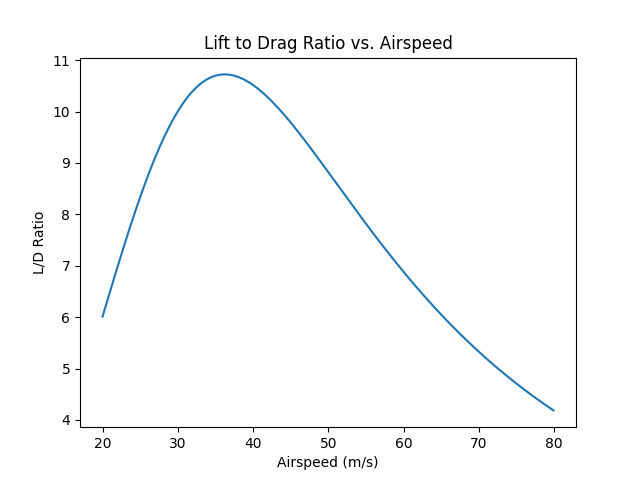
\includegraphics[scale=0.5]{perf_LD} % first figure 
        \caption{Lift-to-Drag ratio}
    \end{minipage}
    \begin{minipage}{0.5\textwidth}
        \centering
        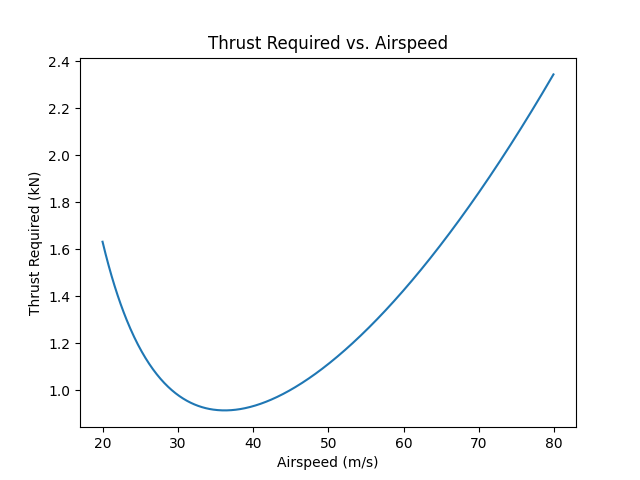
\includegraphics[scale=0.5]{perf_TR} % second figure 
        \caption{Thrust Required}
    \end{minipage}
\end{figure}
\begin{figure}[H]
\centering
    \begin{minipage}{0.45\textwidth}
        \centering
        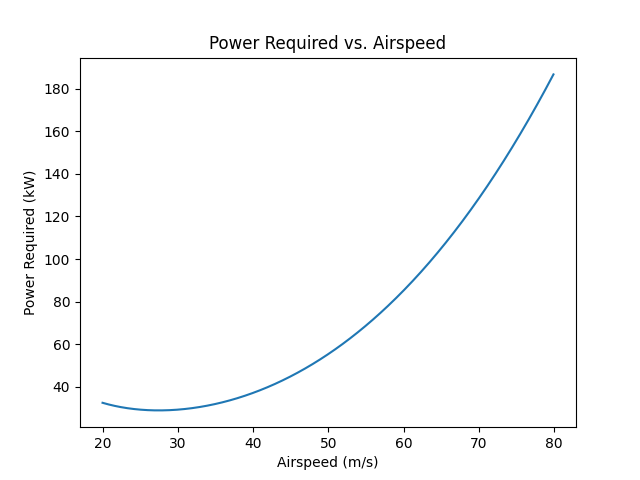
\includegraphics[scale=0.5]{perf_PR} % first figure 
        \caption{Power Required}
    \end{minipage}
    \begin{minipage}{0.5\textwidth}
        \centering
        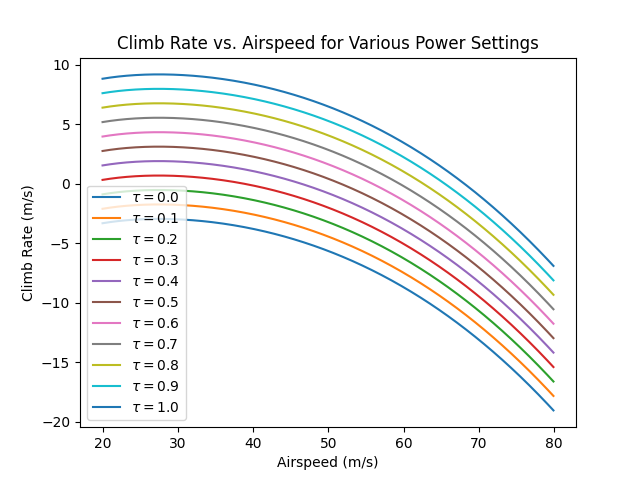
\includegraphics[scale=0.5]{perf_ROC} % second figure 
        \caption{Rate of Climb}
    \end{minipage}
\end{figure}
\begin{figure}[H]
\centering
    \begin{minipage}{0.45\textwidth}
        \centering
        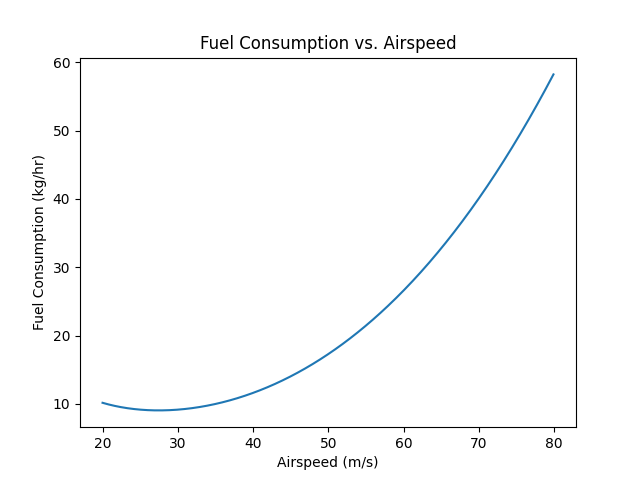
\includegraphics[scale=0.5]{perf_fuel} % first figure 
        \caption{Fuel consumption}
    \end{minipage}
    \begin{minipage}{0.5\textwidth}
        \centering
        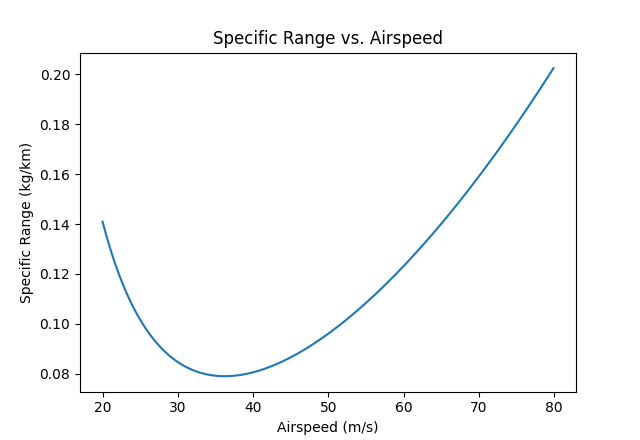
\includegraphics[scale=0.5]{perf_range} % second figure 
        \caption{Specific Range}
    \end{minipage}
\end{figure}

Furthermore, a few data points resulting from the code were compared with experimental data furnished in the aircraft's handbook \cite{cessna}. 
\begin{enumerate}
\item From reference \cite{cessna}, the value of maximum Rate of Climb = 770 fpm = 3.9 m/s at an airspeed value of 73 kts = 37.5 m/s for full throttle ($\tau=1$) at sea level. In comparison, the code was run at sea level (i.e. setting the input density value to 1.22 $kg/m^3$), and the value of maximum rate of climb was found to be 9.1 m/s at an airspeed value of 27.5 m/s. At a speed of 37.5 m/s, the value of climb rate was found to be 8.6 m/s.

\item Next, we attempt to compare Specific Range values. From the handbook \cite{cessna}, under cruise performance, for 75\% power at 8000 feet, Range value is indicated as 485 nm = 898.2 kms, for 40 gallons usable fuel. Considering density of the fuel (Aviation grade straight mineral oil) as 0.88 kg/ltr, the weight of the fuel corresponding to 40 gallons (= 151.4 ltrs) would be around 133 kgs. Dividing the value of range with the weight of fuel consumed, the specific range value = 0.15 kg/km. Also, maximum cruise speed, 75\% power at 8000 feet, is equal to 122 kts = 63 m/s. Running the code taking altitude as 8000 feet, (i.e. setting the input density value to 0.95 $kg/m^3$), value of specific range at an airspeed of 63 m/s is obtained as 0.11 kg/km.

\item Both of the above points show a discrepancy between the experimental value and the code. This deviation can be attributed to the fact that the code does not take actual propulsive efficiencies into account. Further information is needed to determine the actual power available after accounting for the aerodynamic efficiency of the propulsion system.

\item From the results of the code, maximum L/D ratio is around 10.7, and from a different analysis \cite{cessna2} maximum L/D ratio is calculated as 10.9, which shows good agreement.
\end{enumerate}

\begin{thebibliography}{6}
\bibitem{anderson} 
John D. Anderson, Jr.,
\textit{Fundamentals of Aerodynamics}, sixth ed.,
McGraw-Hill Education, New York, 2017.

\bibitem{chow} 
Arnold M. Kuethe and Chuen-Yen Chow,
\textit{Foundations of Aerodynamics Bases of Aerodynamic Design}, fifth ed.,
John Wiley \& Sons, Inc., New York, 1998.

\bibitem{phillips} 
Warren F. Phillips,
\textit{Mechanics of Flight},
John Wiley \& Sons, Inc., New Jersey, 2004.

\bibitem{naca} 
Ira H. Abbott, Albert E. von Doenhoff, and Louis S. Stivers, Jr.,
\textit{Report No. 824, Summary of Airfoil Data},
NACA.

\bibitem{cessna}
\textit{Pilot's Operating Handbook, Cessna Skyhawk 172N},
Cessna Aircraft Company, Kansas, 1977.

\bibitem{cessna2} 
John McIver B.Eng.,
\textit{Cessna Skyhawk Performance Assessment}, Temporal images.
\\\texttt{http//temporal.com.au/c172.pdf}
\end{thebibliography}

\end{document}
